\documentclass[11pt,utf8,notheorems,compress,t]{beamer}
\usepackage{etex}

\usepackage{pgfpages}
\usepackage[export]{adjustbox}

% Workaround for the issue described at
% https://tex.stackexchange.com/questions/164406/beamer-using-href-in-notes.
\newcommand{\fixedhref}[2]{\makebox[0pt][l]{\hspace*{\paperwidth}\href{#1}{#2}}\href{#1}{#2}}

\usepackage[english]{babel}

\usepackage{graphbox}
\usepackage{mathtools}
\usepackage{booktabs}
\usepackage{stmaryrd,wasysym}
\usepackage{bussproofs}
\usepackage{proof}
\usepackage{xspace}
\usepackage{amssymb}
\usepackage{array}
\usepackage{ragged2e}
\usepackage{multicol}
\usepackage{tabto}
\usepackage{xstring}
\usepackage{ifthen}
\usepackage[normalem]{ulem}
\usepackage[all]{xy}
\xyoption{rotate}
\usepackage{tikz}
\usetikzlibrary{calc,shapes,shapes.callouts,shapes.arrows,patterns,fit,backgrounds,decorations.pathmorphing,positioning}
\hypersetup{colorlinks=true}

\newcommand*\circled[1]{\tikz[baseline=(char.base)]{%
  \node[shape=circle,draw,inner sep=1pt] (char) {#1};}}

\DeclareFontFamily{U}{bbm}{}
\DeclareFontShape{U}{bbm}{m}{n}
   {  <5> <6> <7> <8> <9> <10> <12> gen * bbm
      <10.95> bbm10%
      <14.4>  bbm12%
      <17.28><20.74><24.88> bbm17}{}
\DeclareFontShape{U}{bbm}{m}{sl}
   {  <5> <6> <7> bbmsl8%
      <8> <9> <10> <12> gen * bbmsl
      <10.95> bbmsl10%
      <14.4> <17.28> <20.74> <24.88> bbmsl12}{}
\DeclareFontShape{U}{bbm}{bx}{n}
   {  <5> <6> <7> <8> <9> <10> <12> gen * bbmbx
      <10.95> bbmbx10%
      <14.4> <17.28> <20.74> <24.88> bbmbx12}{}
\DeclareFontShape{U}{bbm}{bx}{sl}
   {  <5> <6> <7> <8> <9> <10> <10.95> <12> <14.4> <17.28>%
      <20.74> <24.88> bbmbxsl10}{}
\DeclareFontShape{U}{bbm}{b}{n}
   {  <5> <6> <7> <8> <9> <10> <10.95> <12> <14.4> <17.28>%
      <20.74> <24.88> bbmb10}{}
\DeclareMathAlphabet{\mathbbm}{U}{bbm}{m}{n}
\SetMathAlphabet\mathbbm{bold}{U}{bbm}{bx}{n}

\usepackage{pifont}
\newcommand{\cmark}{\ding{51}}
\newcommand{\xmark}{\ding{55}}
\DeclareSymbolFont{extraup}{U}{zavm}{m}{n}
\DeclareMathSymbol{\varheart}{\mathalpha}{extraup}{86}

\graphicspath{{images/}}

\usepackage[protrusion=true,expansion=true]{microtype}

\setlength\parskip{\medskipamount}
\setlength\parindent{0pt}

\title{Extraction of programs from proofs}
\author{Ingo Blechschmidt}
\date{September 21th, 2022}

\setbeameroption{show notes on second screen}
%\setbeamertemplate{note page}[plain, bg=white!90!black]
\newcommand{\jnote}[2]{\only<#1>{\note{\setlength\parskip{\medskipamount}\footnotesize\justifying#2\par}}}

%\useinnertheme[shadow=true]
\setbeamerfont{block title}{size={}}

\useinnertheme{rectangles}

\usecolortheme{orchid}
\usecolortheme{seahorse}
\definecolor{mypurple}{RGB}{150,0,255}
\setbeamercolor{structure}{fg=mypurple}
\definecolor{myred}{RGB}{150,0,0}
\setbeamercolor*{title}{bg=myred,fg=white}
\setbeamercolor*{titlelike}{bg=myred,fg=white}
\setbeamercolor{frame}{bg=black}

\usefonttheme{serif}
\usepackage[T1]{fontenc}
\usepackage{libertine}

% lifted from https://arxiv.org/abs/1506.08870
\DeclareFontFamily{U}{min}{}
\DeclareFontShape{U}{min}{m}{n}{<-> udmj30}{}
\newcommand\yon{\!\text{\usefont{U}{min}{m}{n}\symbol{'210}}\!}

\newcommand{\A}{\mathcal{A}}
\newcommand{\B}{\mathcal{B}}
\newcommand{\C}{\mathcal{C}}
\newcommand{\M}{\mathcal{M}}
\renewcommand{\AA}{\mathbb{A}}
\newcommand{\BB}{\mathbb{B}}
\newcommand{\pp}{\mathbbm{p}}
\newcommand{\MM}{\mathbb{M}}
\newcommand{\E}{\mathcal{E}}
\newcommand{\F}{\mathcal{F}}
\newcommand{\FF}{\mathbb{F}}
\newcommand{\G}{\mathcal{G}}
\newcommand{\J}{\mathcal{J}}
\newcommand{\GG}{\mathbb{G}}
\renewcommand{\O}{\mathcal{O}}
\newcommand{\K}{\mathcal{K}}
\newcommand{\NN}{\mathbb{N}}
\newcommand{\QQ}{\mathbb{Q}}
\newcommand{\RR}{\mathbb{R}}
\newcommand{\TT}{\mathbb{T}}
\newcommand{\PP}{\mathbb{P}}
\newcommand{\ZZ}{\mathbb{Z}}
\newcommand{\CC}{\mathbb{C}}
\renewcommand{\P}{\mathcal{P}}
\newcommand{\aaa}{\mathfrak{a}}
\newcommand{\ppp}{\mathfrak{p}}
\newcommand{\fff}{\mathfrak{f}}
\newcommand{\defeq}{\vcentcolon=}
\newcommand{\defeqv}{\vcentcolon\equiv}
\newcommand{\Sh}{\mathrm{Sh}}
\newcommand{\GL}{\mathrm{GL}}
\newcommand{\Zar}{\mathrm{Zar}}
\newcommand{\op}{\mathrm{op}}
\newcommand{\Set}{\mathrm{Set}}
\newcommand{\Eff}{\mathrm{Ef{}f}}
\newcommand{\Sch}{\mathrm{Sch}}
\newcommand{\Aff}{\mathrm{Aff}}
\newcommand{\Ring}{\mathrm{Ring}}
\newcommand{\LocRing}{\mathrm{LocRing}}
\newcommand{\LRS}{\mathrm{LRS}}
\newcommand{\Hom}{\mathrm{Hom}}
\newcommand{\Spec}{\mathrm{Spec}}
\newcommand{\lra}{\longrightarrow}
\newcommand{\RelSpec}{\operatorname{Spec}}
\renewcommand{\_}{\mathpunct{.}\,}
\newcommand{\?}{\,{:}\,}
\newcommand{\speak}[1]{\ulcorner\text{\textnormal{#1}}\urcorner}
\newcommand{\ul}[1]{\underline{#1}}
\newcommand{\affl}{\ensuremath{{\ul{\ensuremath{\AA}}^1}}}
\newcommand{\Ll}{\text{iff}}
\newcommand{\inv}{inv.\@}
\newcommand{\seq}[1]{\mathrel{\vdash\!\!\!_{#1}}}
\newcommand{\hg}{\mathbin{:}}  % homogeneous coordinates

\setbeamertemplate{blocks}[rounded][shadow=false]

\newenvironment{indentblock}{%
  \list{}{\leftmargin\leftmargin}%
  \item\relax
}{%
  \endlist
}

% Adapted from https://latex.org/forum/viewtopic.php?t=2251 (Stefan Kottwitz)
\newenvironment<>{hilblock}{
  \begin{center}
    \begin{minipage}{9.05cm}
      \setlength{\textwidth}{9.05cm}
      \begin{actionenv}#1
        \def\insertblocktitle{}
        \par
        \usebeamertemplate{block begin}}{
        \par
        \usebeamertemplate{block end}
      \end{actionenv}
    \end{minipage}
  \end{center}}

\newenvironment{changemargin}[2]{%
  \begin{list}{}{%
    \setlength{\topsep}{0pt}%
    \setlength{\leftmargin}{#1}%
    \setlength{\rightmargin}{#2}%
    \setlength{\listparindent}{\parindent}%
    \setlength{\itemindent}{\parindent}%
    \setlength{\parsep}{\parskip}%
  }%
  \item[]}{\end{list}}

\tikzset{
  invisible/.style={opacity=0,text opacity=0},
  visible on/.style={alt={#1{}{invisible}}},
  alt/.code args={<#1>#2#3}{%
    \alt<#1>{\pgfkeysalso{#2}}{\pgfkeysalso{#3}}}
}

\newcommand{\pointthis}[3]{%
  \tikz[remember picture,baseline]{
    \node[anchor=base,inner sep=0,outer sep=0] (#2) {#2};
    \node[visible on=#1,overlay,rectangle callout,rounded corners,callout relative pointer={(0.3cm,0.5cm)},fill=blue!20] at ($(#2.north)+(-0.1cm,-1.1cm)$) {#3};
  }%
}

\tikzset{
  invisible/.style={opacity=0,text opacity=0},
  visible on/.style={alt={#1{}{invisible}}},
  alt/.code args={<#1>#2#3}{%
    \alt<#1>{\pgfkeysalso{#2}}{\pgfkeysalso{#3}}}
}

\newcommand{\hcancel}[5]{%
  \tikz[baseline=(tocancel.base)]{
    \node[inner sep=0pt,outer sep=0pt] (tocancel) {#1};
    \draw[red!80, line width=0.4mm] ($(tocancel.south west)+(#2,#3)$) -- ($(tocancel.north east)+(#4,#5)$);
  }%
}

\newcommand{\explain}[7]{%
  \tikz[remember picture,baseline]{
    \node[anchor=base,inner sep=2pt,outer sep=0,fill=#3,rounded corners] (label) {#1};
    \node[anchor=north,visible on=<#2>,overlay,rectangle callout,rounded corners,callout
    relative pointer={(0.0cm,0.5cm)+(0.0cm,#6)},fill=#3] at ($(label.south)+(0,-0.3cm)+(#4,#5)$) {#7};
  }%
}

\newcommand{\explainstub}[2]{%
  \tikz[remember picture,baseline]{
    \node[anchor=base,inner sep=2pt,outer sep=0,fill=#2,rounded corners] (label) {#1};
  }%
}

\newcommand{\squiggly}[1]{%
  \tikz[remember picture,baseline]{
    \node[anchor=base,inner sep=0,outer sep=0] (label) {#1};
    \draw[thick,color=red!80,decoration={snake,amplitude=0.5pt,segment
    length=3pt},decorate] ($(label.south west) + (0,-2pt)$) -- ($(label.south east) + (0,-2pt)$);
  }%
}

% Adapted from https://latex.org/forum/viewtopic.php?t=2251 (Stefan Kottwitz)
\newenvironment<>{varblock}[2]{\begin{varblockextra}{#1}{#2}{}}{\end{varblockextra}}
\newenvironment<>{varblockextra}[3]{
  \begin{center}
    \begin{minipage}{#1}
      \begin{actionenv}#4
        {\centering \hil{#2}\par}
	\def\insertblocktitle{}%\centering #2}
        \def\varblockextraend{#3}
	\usebeamertemplate{block begin}}{
        \par
        \usebeamertemplate{block end}
        \varblockextraend
      \end{actionenv}
    \end{minipage}
  \end{center}}

\setbeamertemplate{headline}{}

\setbeamertemplate{frametitle}{%
  \vskip0.5em%
  \leavevmode%
  \begin{beamercolorbox}[dp=1ex,center]{}%
    \begin{tikzpicture}
      \def\R{8pt}
      \node (title) {\hil{{\large\,\!\insertframetitle}}};
      \begin{pgfonlayer}{background}
        \draw[decorate, very thick, draw=mypurple!30]
          ($(title.south west) + (\R, 0)$) arc(270:180:\R) --
          ($(title.north west) + (0, -\R)$) arc(180:90:\R) --
          ($(title.north east) + (-\R, 0)$) arc(90:0:\R) --
          ($(title.south east) + (0, \R)$) arc(0:-90:\R) --
          cycle;
      \end{pgfonlayer}
    \end{tikzpicture}
  \end{beamercolorbox}%
  \vskip-0.2em%
}

\setbeamertemplate{navigation symbols}{}

\newcounter{framenumberpreappendix}
\newcommand{\backupstart}{
  \setcounter{framenumberpreappendix}{\value{framenumber}}
}
\newcommand{\backupend}{
  \addtocounter{framenumberpreappendix}{-\value{framenumber}}
  \addtocounter{framenumber}{\value{framenumberpreappendix}}
}

\newcommand{\insertframeextra}{}
\setbeamertemplate{footline}{%
  \begin{beamercolorbox}[wd=\paperwidth,ht=2.25ex,dp=1ex,right,rightskip=1mm,leftskip=1mm]{}%
    % \inserttitle
    \hfill
    \insertframenumber\insertframeextra\,/\,\inserttotalframenumber
  \end{beamercolorbox}%
  \vskip0pt%
}


\newcommand{\hil}[1]{{\usebeamercolor[fg]{item}{\textbf{#1}}}}
\newcommand{\bad}[1]{\textcolor{red!90}{\textnormal{#1}}}
\newcommand{\good}[1]{\textcolor{mypurple}{\textnormal{#1}}}

\newcommand{\bignumber}[1]{%
  \renewcommand{\insertenumlabel}{#1}\scalebox{1.2}{\!\usebeamertemplate{enumerate item}\!}
}
\newcommand{\normalnumber}[1]{%
  {\renewcommand{\insertenumlabel}{#1}\!\usebeamertemplate{enumerate item}\!}
}
\newcommand{\bigheart}{
\includegraphics{heart}}

\newcommand{\subhead}[1]{{\centering\textcolor{gray}{\hrulefill}\quad\textnormal{#1}\quad\textcolor{gray}{\hrulefill}\par}}

\newcommand{\badbox}[1]{\colorbox{red!30}{#1}}
\newcommand{\infobox}[1]{\colorbox{yellow!70}{\color{black}#1}}
\newcommand{\grayline}{\textcolor{gray}{\hspace*{-3em}\hrulefill\hspace*{-3em}}}
\newcommand{\notnot}{\emph{not~not}\xspace}

\begin{document}

\addtocounter{framenumber}{-1}

%\setbeamertemplate{headline}{\mynav{gray}{gray}{gray}}

{\usebackgroundtemplate{\begin{minipage}{\paperwidth}\vspace*{1.59cm}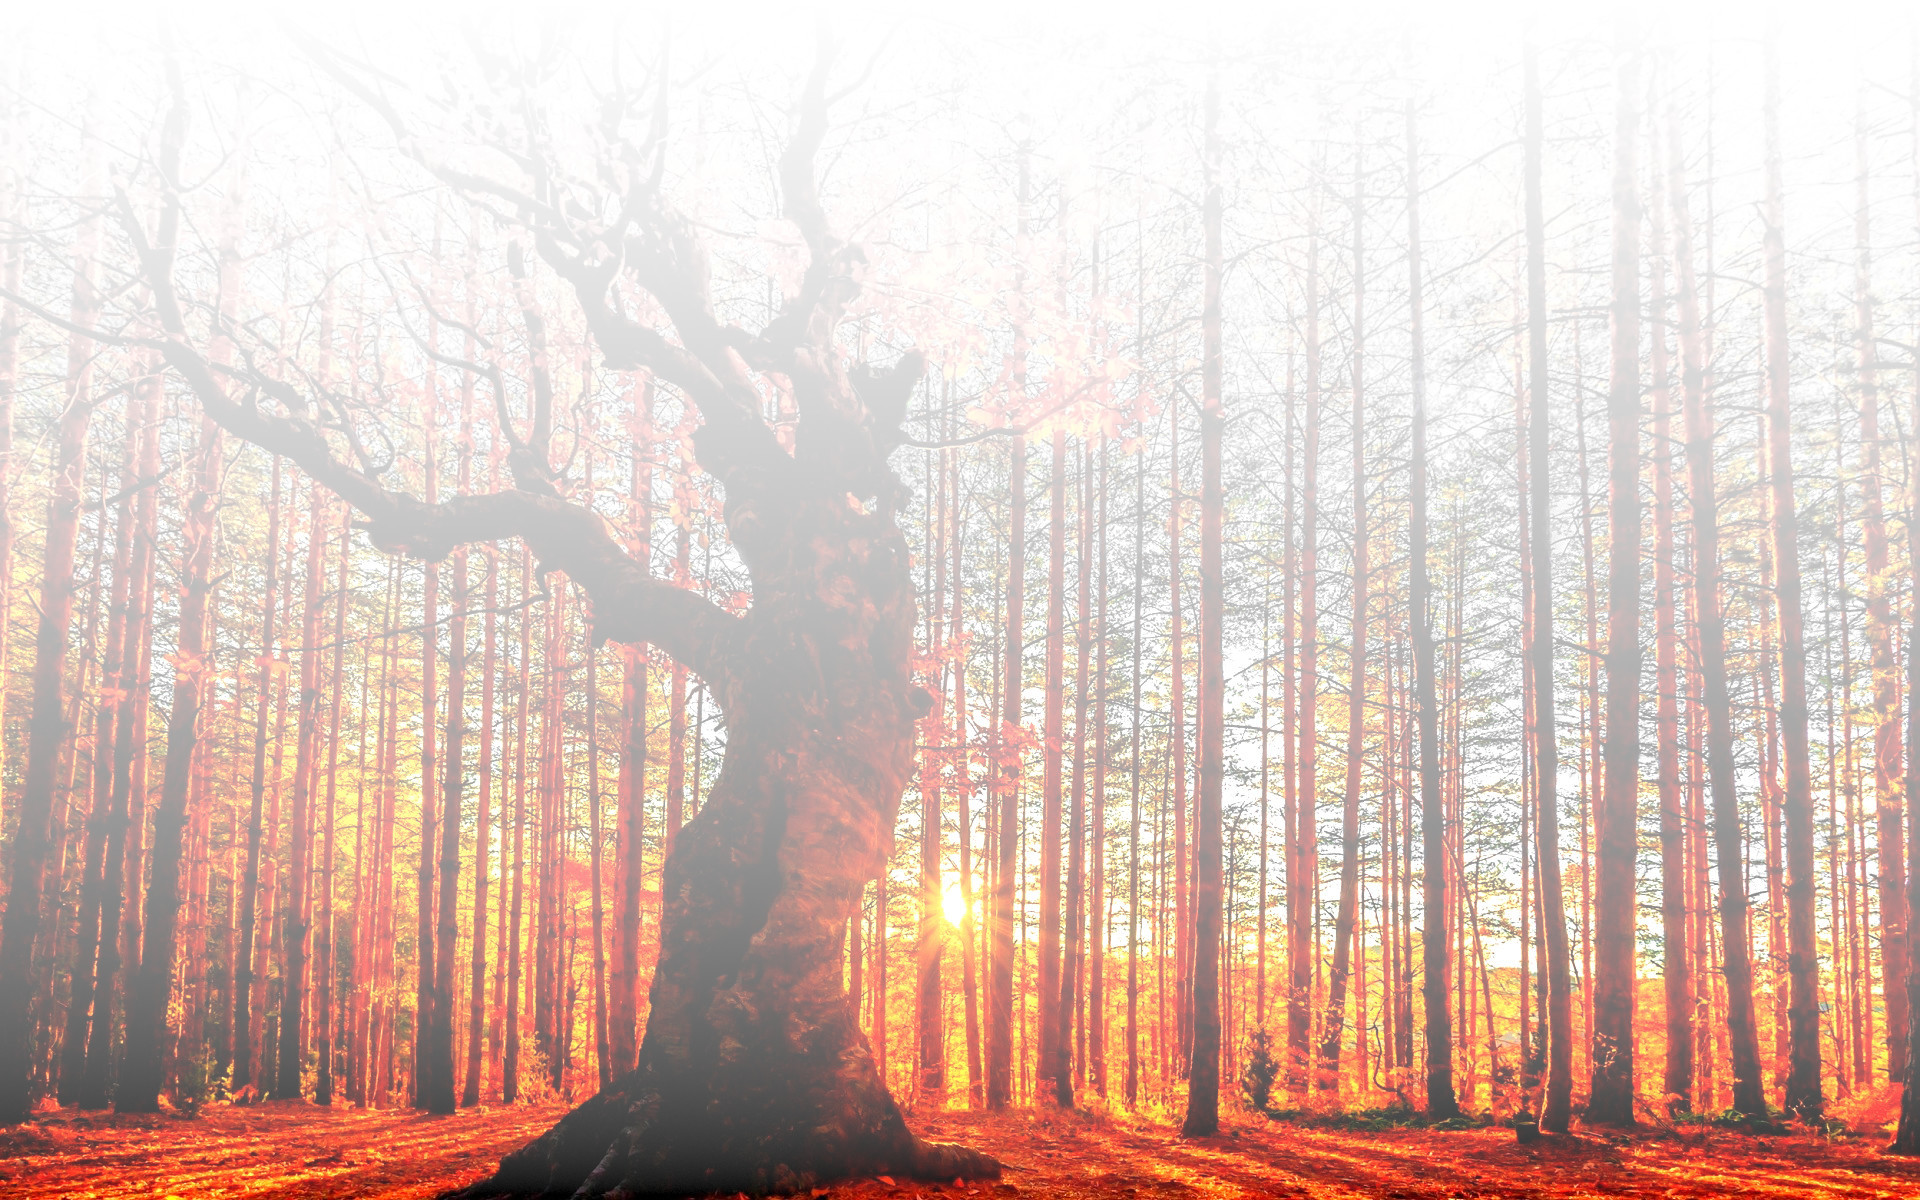
\includegraphics[width=\paperwidth]{forest-light}\end{minipage}}
\definecolor{mypurple}{RGB}{253,73,34}
\begin{frame}[c]
  \centering

  \bigskip
  \bigskip
  \bigskip
  \bigskip

  \scriptsize
  \textit{-- an invitation --}

  \setbeamercolor{block body}{bg=black!100}
  \begin{block}{}
    \centering\normalsize\color{white}
    \hil{Extraction} of \hil{programs} from \hil{proofs}
  \end{block}

  \bigskip
  \bigskip
  \bigskip
  \bigskip
  \bigskip
  \bigskip
  \bigskip

  Autumn school on \\
  \emph{Proof and Computation} \\
  in Fischbachau \\
  \ \\
  September 26th to October 1st, 2022

  Ingo Blechschmidt \\
  University of Augsburg
  \par
\end{frame}}

{\usebackgroundtemplate{\begin{minipage}{\paperwidth}\vspace*{5.95cm}
\includegraphics[width=\paperwidth]{fr1-lighter}\end{minipage}}
\begin{frame}{}
  \jnote{1-5}{
    From the displayed proof of Euclid's theorem, we can read off an algorithm
    for computing arbitrarily large primes. There is a deeper reason to that:
    The proof is \emph{constructive}, and from \emph{every} constructive proof
    we can extract a corresponding program. One way to formally state and prove
    this meta-statement is by \emph{realizability theory}, the subject of the
    first lecture.
  }

  \jnote{4-5}{
    In addition to the displayed applications of realizability theory,
    personally I'm intrigued by it for mostly the following reasons:
    (1)~Realizability elucidates the interplay between constructive and
    computable mathematics. (2)~Realizability is a useful guide for pursuing
    the question whether two given proofs are ``secretly the same'': Do they
    have the same computational content? (3)~Realizability theory provides us
    with a host of tantalizing anti-classical models of constructive
    mathematics.
  }

  \jnote{5-5}{
    In the second lecture, we will turn to extracting programs from
    \emph{classical} proofs. We will do so by transforming classical proofs
    into constructive ones and then applying the tools of the first lecture.
    Amazingly, the displayed classical proof and others like it do have
    constructive content---even though it is constructively and computably
    impossible to determine minimal values of infinite sequences.
  }

  \jnote{6-}{
    Finally, in the third lecture we will learn how to extract constructive
    content from certain kinds of \emph{invalid} proofs---those which use the
    preposterous assumption that every set is countable.

    The methods presented in the second and in the third lecture are deeply
    related to the \emph{dynamical approach to algebra} reported on in Stefan
    Neuwirth's course. Coherent (and geometric) logic as in Marc Bezem's course
    also plays an important role in this toolbox. It is greatly informed by a
    categorical analysis as provided in Steve Awodey's course, particularly so
    for the third lecture. The first and the second lecture overlap with
    Chuangjie Xu's course, particularly regarding the
    double-negation translation.

    This course is set in an informal constructive metatheory. Formalization
    would both be possible in type theory as in Fredrik Nordvall-Forsberg's
    course or in constructive set theory as in Hajime Ishihare's course.
    All appeals to the transfinite such as by the law of excluded middle or
    by the axiom of choice will be explicitly pointed out. For primers to
    constructive mathematics, enjoy
    \fixedhref{https://video.ias.edu/members/1213/0318-AndrejBauer}{Andrej
    Bauer's 2013 IAS talk}, its \fixedhref{xxx}{written version} or
    \fixedhref{xxx}{these course notes}.
  }

  \medskip
  \textbf{Thm.}
  For every number~$n \in \NN$, there is a prime larger than~$n$.

  {\emph{Proof.} Any prime factor of~$n! + 1$ will do.\par}
  \medskip
  \pause

  {\centering\emph{``Every constructive theorem has a computable witness.''}
  \pause
  \[
    \begin{array}{c@{\qquad}c@{\qquad}c}
      \mathrm{HA} \vdash \varphi &\Longrightarrow&
      \exists e\_ e \Vdash \varphi \\
      \text{\small constructive proof} &\longmapsto&
      \text{\small realizer}
    \end{array}
  \]}
  \pause
  \vspace*{-2.2em}

  \begin{columns}
    \begin{column}{0.45\textwidth}
      \begin{itemize}
        \item Integrated developments \\ \emph{SAT checking, \ldots}
        \item Computability theory \\ \emph{induction $\widehat{=}$ recursion, \ldots}
      \end{itemize}
    \end{column}

    \hspace*{-1em}
    \begin{column}{0.65\textwidth}
      \begin{itemize}
        \item Metatheory of constructive systems \\ \emph{provability results, \ldots}
        \item Philosophy of proof and computation \\ \emph{realizability in the real world, \ldots}
      \end{itemize}
    \end{column}
  \end{columns}

  \grayline
  \pause

  \justifying
  \textbf{Thm.} Every infinite sequence~$\alpha : \NN \to \NN$ is \emph{good}
  in that there are numbers~$i < j$ such that~$\alpha(i) \leq \alpha(j)$.

  {\emph{Proof.} By~\badbox{\textsc{lem}}, there is a minimal value~$\alpha(i)$.
  Set~$j \defeq i + 1$.\par}

  {\centering\emph{``\textnormal{Every} theorem has a computable* witness.''} \\ \scriptsize
  * with monadic side effects\par}
\end{frame}}

% 
\includegraphics[width=3cm]{lovelace-babbage}
% 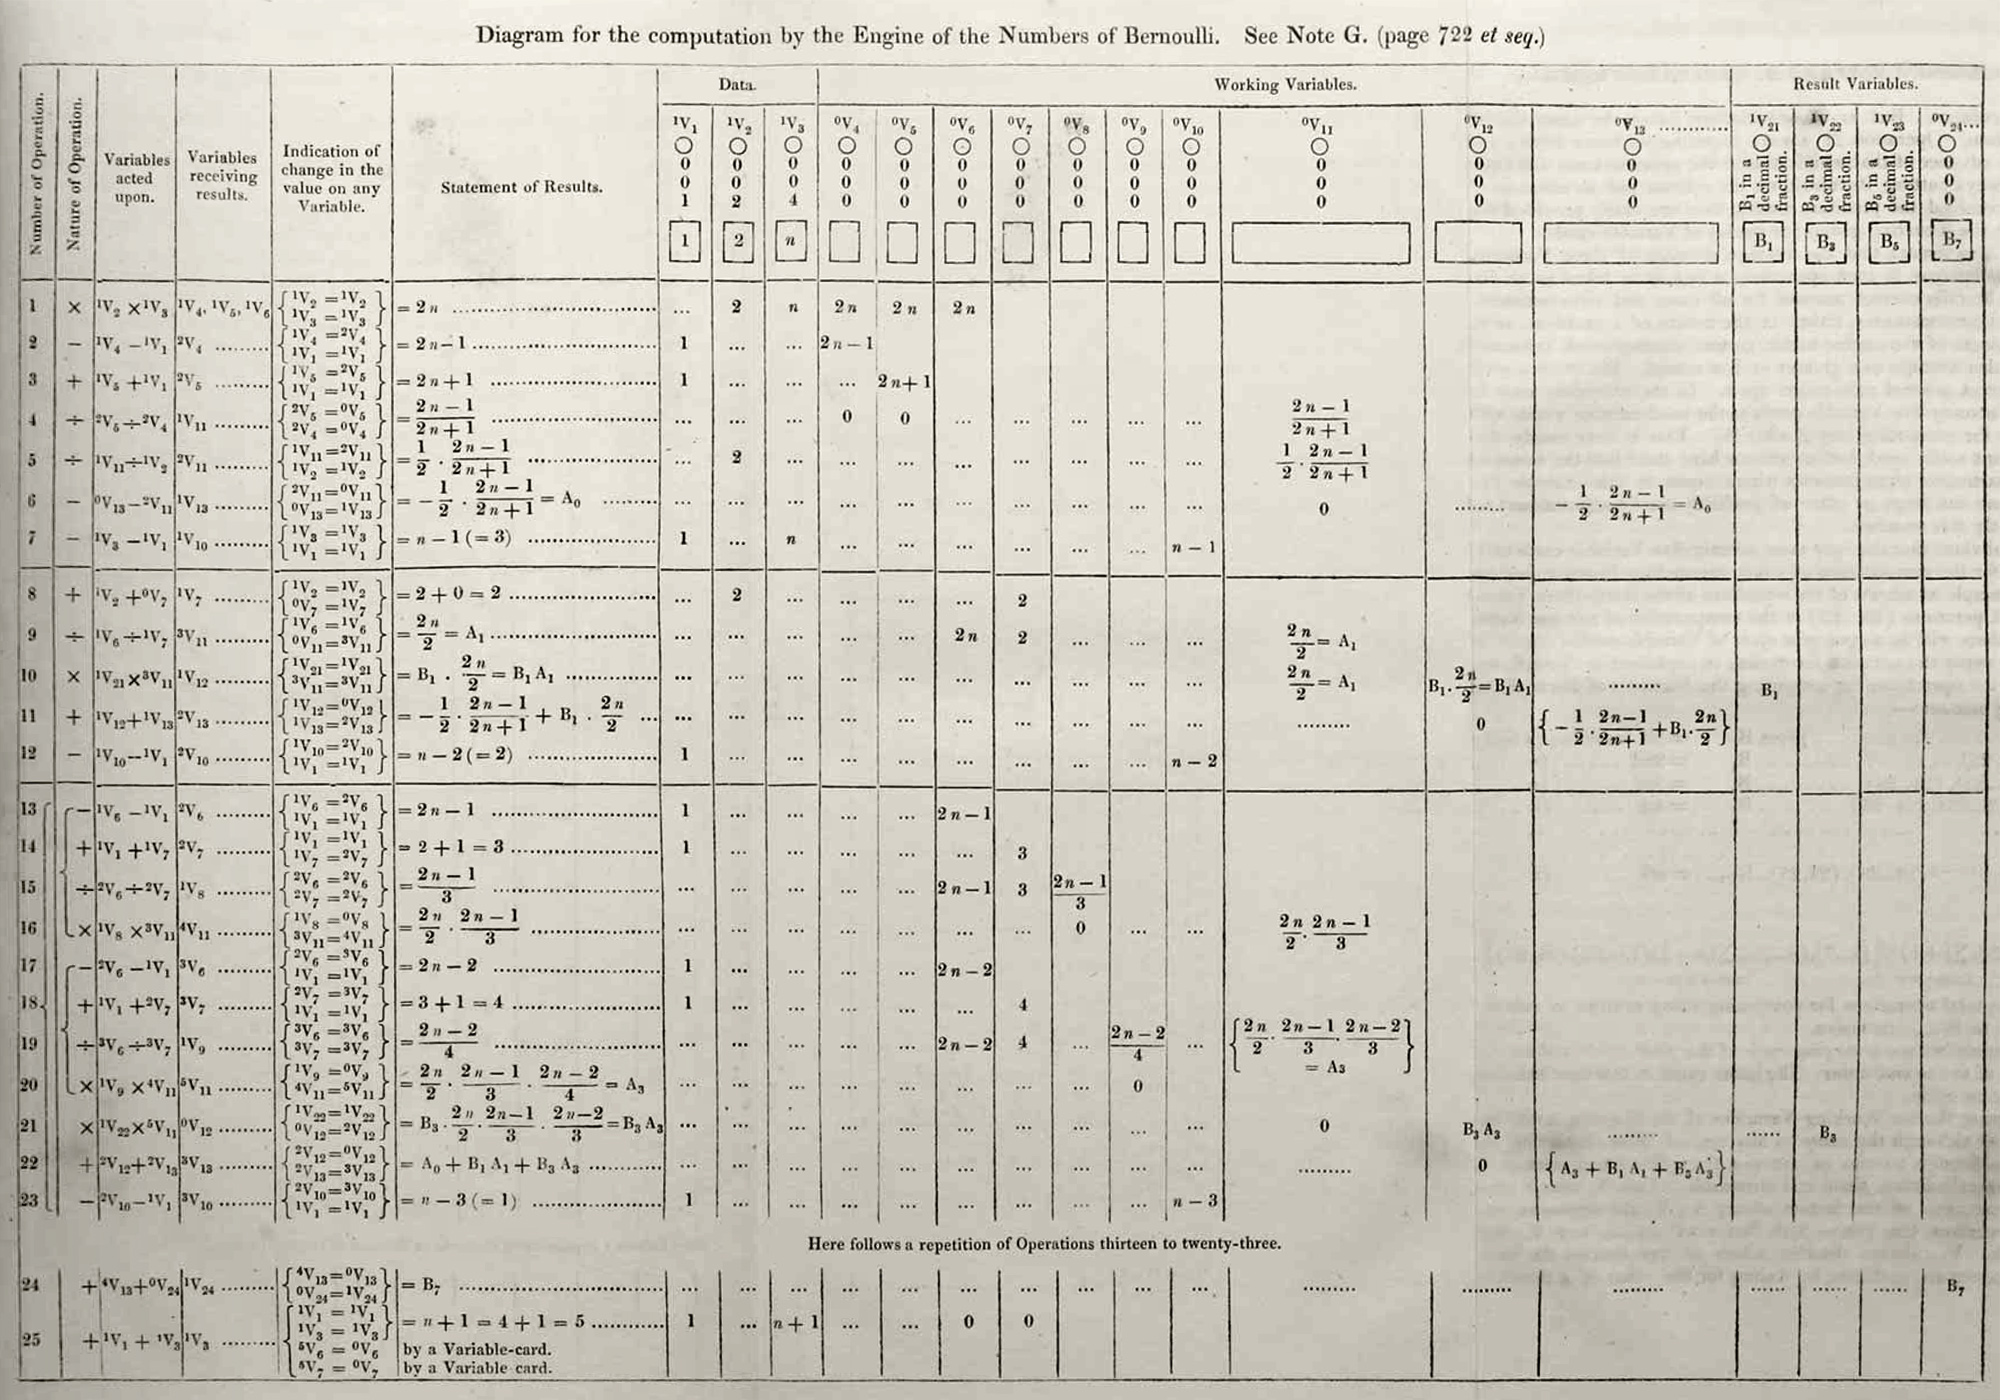
\includegraphics[width=3cm]{first-program}
\addtocounter{framenumber}{-1}
{\usebackgroundtemplate{\begin{minipage}{\paperwidth}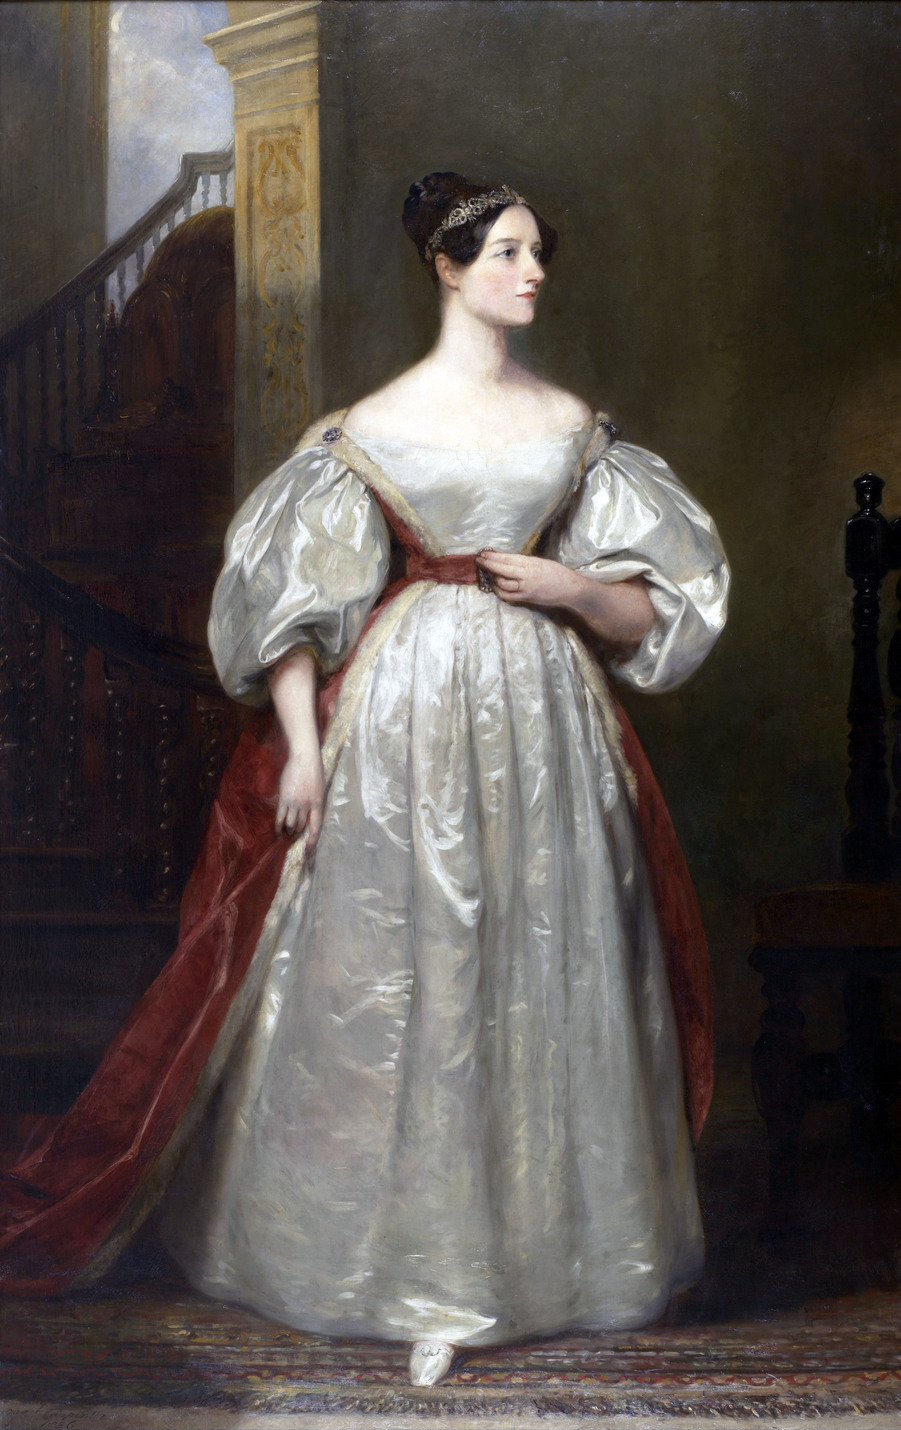
\includegraphics[height=\paperheight,valign=t]{ada-lovelace}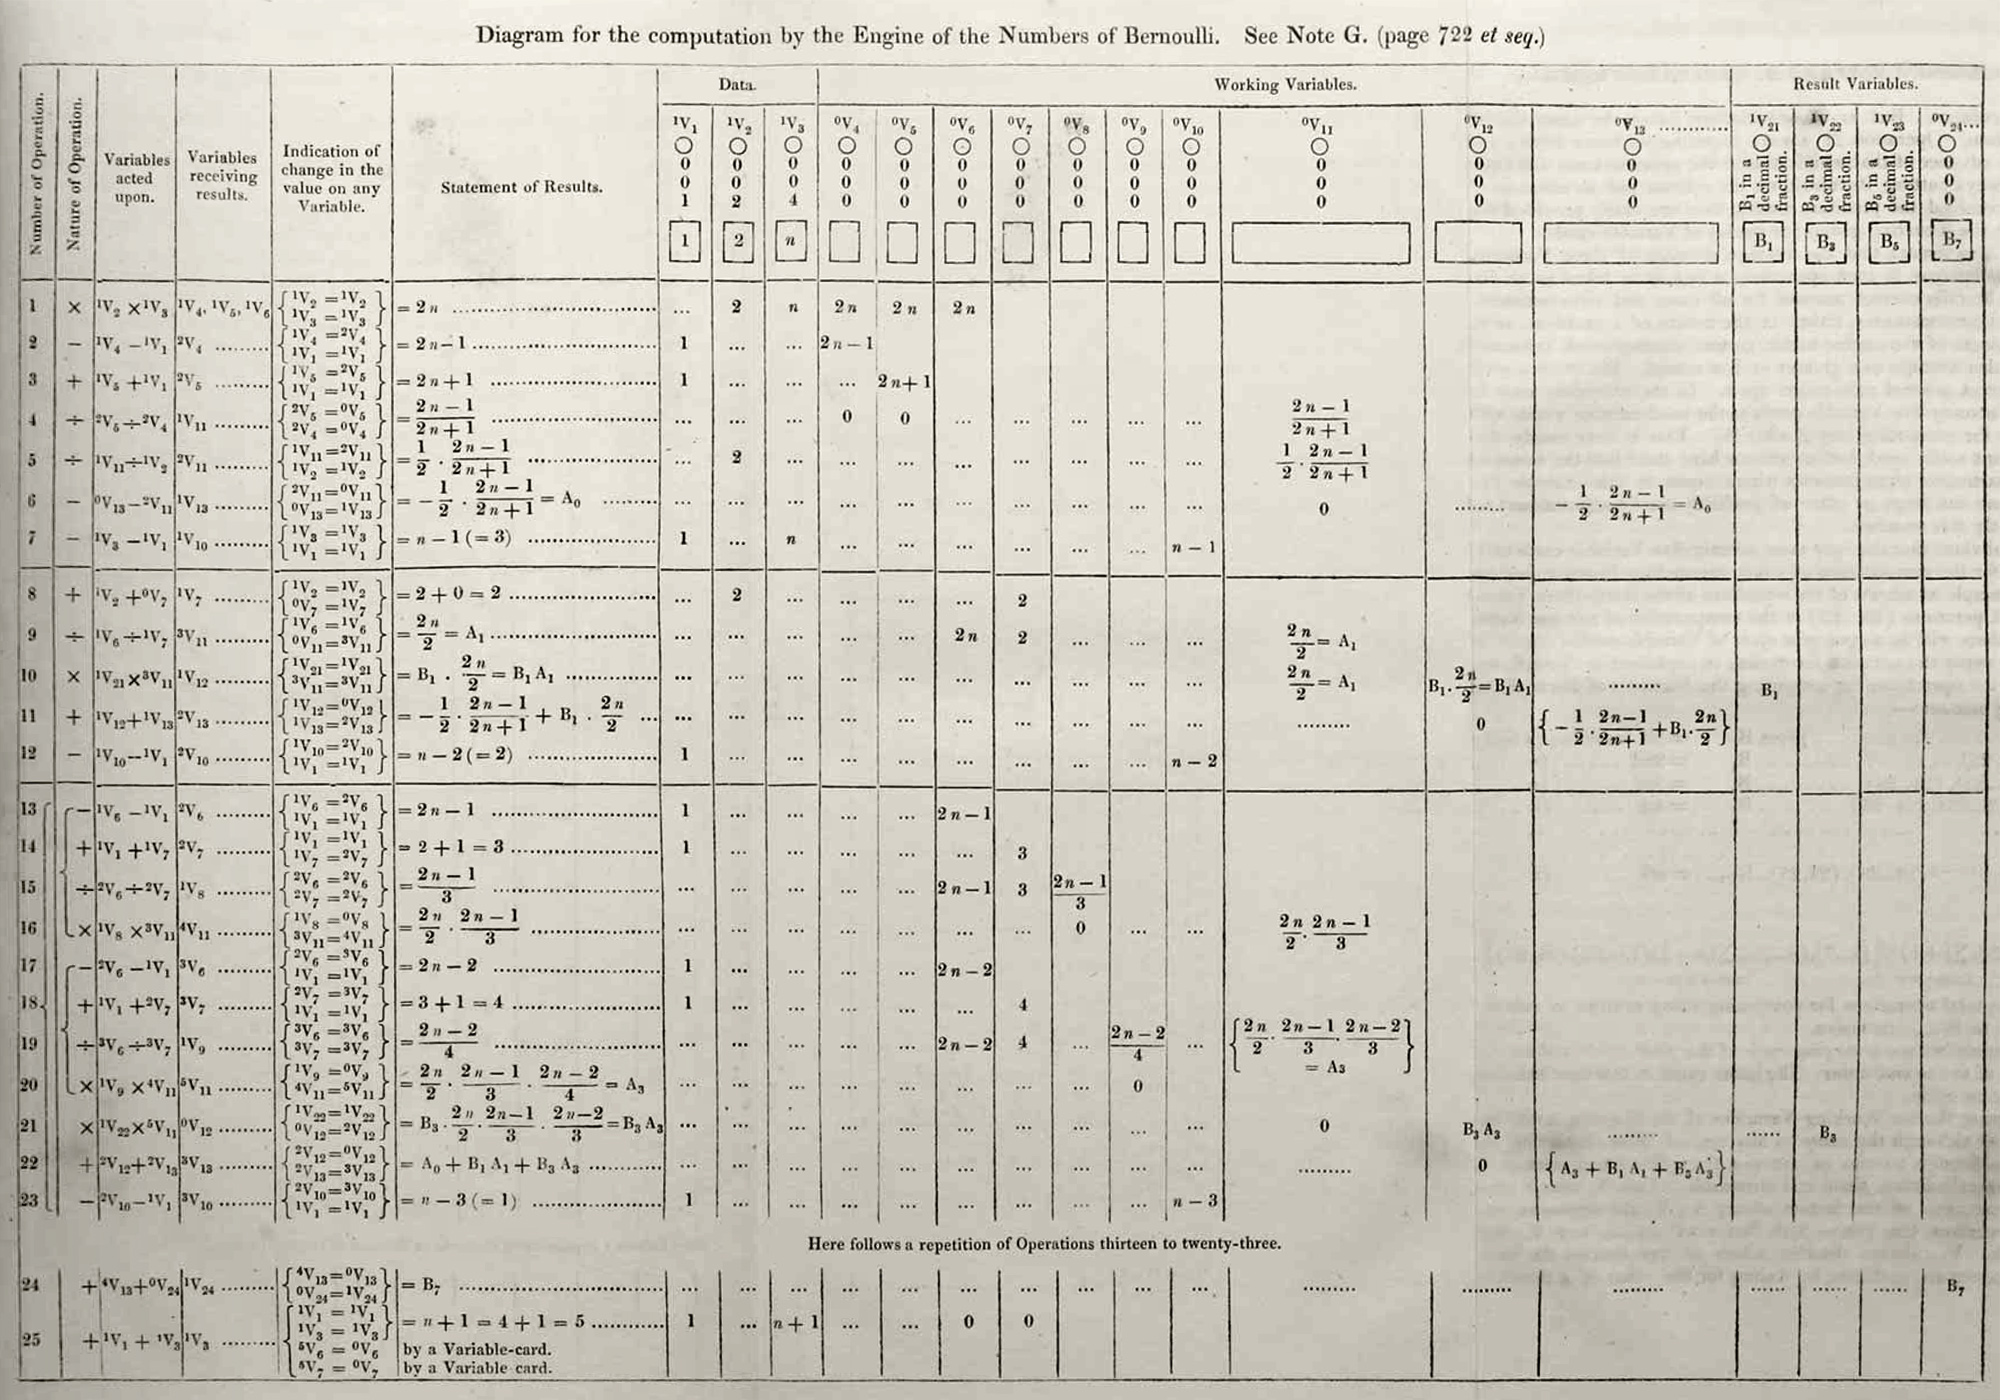
\includegraphics[width=8cm,valign=t]{first-program}\end{minipage}}
\begin{frame}[plain]
  \vspace*{6cm}\hspace*{6cm}\begin{minipage}{4.7cm}
    \huge\hil{Ada Lovelace},

    \Large
    the world's first \\
    computer programmer
    \medskip

    * 1815 \ \ † 1852
  \end{minipage}

  \jnote{1}{
    This year we will celebrate the 207th birthday of Ada Lovelace, pioneer in
    computing.

    It is astonishing what she started and what long way we have come!

    Perhaps you would enjoy the graphic novel \emph{The Thrilling Adventures of
    Lovelace and Babbage} in her honor.
  }
\end{frame}}


\section{Realizability theory}

\begin{frame}
  \centering\bigskip
  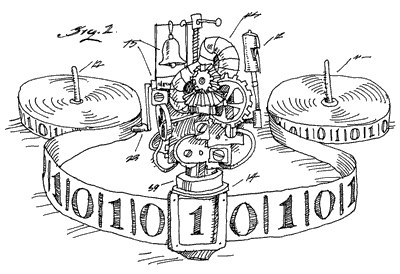
\includegraphics[height=9.5em]{turing-machine}
  \medskip

  \large Lecture I: \\
  \hil{Realizability theory}

  \normalsize

  \emph{for extracting programs from constructive proofs}

  \jnote{1}{
    Monika Seisenberger has
    \fixedhref{https://www.proofsociety.org/wp-content/uploads/2018/09/ProgramExtraction_slides.pdf}{many
    and more detailed} slides on this topic.

    For a written primer to realizability theory, see
    \fixedhref{http://math.andrej.com/asset/data/c2c.pdf}{Andrej Bauer's course
    notes} and the notes by
    \fixedhref{https://www2.mathematik.tu-darmstadt.de/~streicher/REAL/REAL.pdf}{Thomas
    Streicher}.
  }
\end{frame}

\begin{frame}{Heyting arithmetic}
  The \hil{language of arithmetic} has
  \begin{itemize}
    \item as its single sort: $N$
    \item as function symbols: $0$, $S$, $+$, $\cdot$
    \item as its single relation symbol: $=$
  \end{itemize}

  \hil{Heyting arithmetic} has as axioms (the universal closure of)
  \begin{align*}
    &&& \neg(0 = Sx) \\
    &&& S(x) = S(y) \Rightarrow x = y \\
    x + 0 &= x &&&
    x \cdot 0 &= 0 \\
    x + S(y) &= S(x+y) &&&
    x \cdot S(y) &= (x \cdot y) + x
  \end{align*}
  together with the \hil{induction scheme} (one axiom for each
  formula~$\varphi$)
  \[
    \varphi(0) \wedge \bigl(\forall x\?N\_ \varphi(x) \Rightarrow
    \varphi(S(x))\bigr) \quad\Longrightarrow\quad \forall x\?N\_ \varphi(x)
  \]
  and the rules of \hil{sequence calculus}.

  \jnote{1}{
    Heyting arithmetic is a convenient base theory for a constructive analysis
    of arithmetic. It has exactly the same axioms as Peano arithmetic, only
    that HA is set in intuitionistic logic while PA adds the law of excluded
    middle.

    As is common, we define negation~``$\neg\varphi$'' as a shorthand for the
    implication~``$\varphi \Rightarrow \bot$''.

    HA is often expanded to HA\textsuperscript{$\omega$}, \emph{higher-order
    Heyting arithmetic}, which includes sorts, term constructors and
    appropriate rules for function types such as~$N^N$ and $N^{(N^N)}$.

    In its original form, realizability theory is only concernced with
    extracting computational witnesses from HA-proofs; however it is fruitfully
    extended to all of~HA\textsuperscript{$\omega$}, and we will also glimpse
    into this higher-order extension. (NB: HA\textsuperscript{$\omega$} is
    conservative over~HA, and one way to show this is by realizability.)
  }
\end{frame}

\begin{frame}{Sequence calculus}
  \begin{center}
    \vspace{-0.5em}
    \phantom{a}\hfill
    \AxiomC{$\phantom{\seq{\vec x}}$}\UnaryInfC{$\varphi \seq{\vec x} \varphi$}\DisplayProof\hfill
    \AxiomC{$\varphi \seq{\vec x} \psi$}\UnaryInfC{$\varphi[\vec s/\vec x]
    \seq{\vec y} \psi[\vec s/\vec x]$}\DisplayProof\hfill
    \AxiomC{$\varphi \seq{\vec x} \psi$}\AxiomC{$\psi \seq{\vec x}
    \chi$}\BinaryInfC{$\varphi \seq{\vec x} \chi$}\DisplayProof
    \phantom{a}\hfill
    \bigskip\medskip

    \phantom{a}\hfill
    \AxiomC{$\phantom{\seq{\vec x}}$}\UnaryInfC{$\varphi \seq{\vec x} \top$}\DisplayProof\hfill
    \AxiomC{$\phantom{\seq{\vec x}}$}\UnaryInfC{$\varphi \wedge \psi \seq{\vec x} \varphi$}\DisplayProof\hfill
    \AxiomC{$\phantom{\seq{\vec x}}$}\UnaryInfC{$\varphi \wedge \psi \seq{\vec x} \psi$}\DisplayProof\hfill
    \AxiomC{$\varphi \seq{\vec x} \psi$}\AxiomC{$\varphi \seq{\vec x} \chi$}\BinaryInfC{$\varphi \seq{\vec x} \psi \wedge \chi$}\DisplayProof
    \phantom{a}\hfill
    \bigskip\medskip

    \phantom{a}\hfill
    \AxiomC{$\phantom{\seq{\vec x}}$}\UnaryInfC{$\bot \seq{\vec x} \varphi$}\DisplayProof\hfill
    \AxiomC{$\phantom{\seq{\vec x}}$}\UnaryInfC{$\varphi \seq{\vec x} \varphi \vee \psi$}\DisplayProof\hfill
    \AxiomC{$\phantom{\seq{\vec x}}$}\UnaryInfC{$\psi \seq{\vec x} \varphi \vee \psi$}\DisplayProof\hfill
    \AxiomC{$\varphi \seq{\vec x} \chi$}\AxiomC{$\psi \seq{\vec x} \chi$}\BinaryInfC{$\varphi \vee \psi \seq{\vec x} \chi$}\DisplayProof
    \phantom{a}\hfill
    \bigskip\medskip

    \phantom{a}\hfill
    \Axiom$\varphi \wedge \psi\ \fCenter\seq{\vec x} \chi$
    \doubleLine
    \UnaryInf$\varphi\ \fCenter\seq{\vec x} \psi \Rightarrow \chi$
    \DisplayProof
    \phantom{a}\hfill
    \bigskip\medskip

    \phantom{a}\hfill
    \Axiom$\varphi\ \fCenter\seq{\vec x, y} \psi$
    \doubleLine
    \UnaryInf$\exists y\?Y\_\! \varphi\ \fCenter\seq{\vec x} \psi$
    \DisplayProof
    {\tiny ($y$ not occurring in~$\psi$)}
    \hfill
    \Axiom$\varphi\ \fCenter\seq{\vec x, y} \psi$
    \doubleLine
    \UnaryInf$\varphi\ \fCenter\seq{\vec x\phantom{, y}} \forall y\?Y\_\! \psi$
    \DisplayProof
    {\tiny ($y$ not occurring in~$\varphi$)}
    \hfill\phantom{a}

    \phantom{a}\hfill
    \AxiomC{$\phantom{\seq{\vec x}}$}
    \UnaryInfC{$\top \seq{x} x = x$}
    \DisplayProof
    \hfill
    \AxiomC{$\phantom{\seq{\vec x}}$}
    \UnaryInfC{$(\vec x = \vec y) \wedge \varphi \seq{\vec z} \varphi[\vec y/\vec x]$}
    \DisplayProof
    \hfill\phantom{a} \\[0.5em]
    (``$\vec x = \vec y\,$'' is short for~``$x_1 = y_1 \wedge \cdots \wedge x_n =
    y_n$''.)
  \end{center}
\end{frame}

\newcommand{\realizes}{\Vdash}

\begin{frame}{Number realizability}
  \jnote{1}{
    A statement~$\varphi$ is \emph{realizable}, written~``$\realizes\varphi$'',
    iff it has a \emph{realizer}, a number~$e \in \NN$ such that~$e \realizes
    \varphi$. The recursive rules governing which numbers~$e$ are deemed to be
    a realizer of~$\varphi$ make use of \emph{Kleene's original partial combinatory
    algebra}, the natural numbers equipped with the following partial binary
    operation~$({\cdot})$: $e \cdot n$ is the result of applying the
    input~$n$ to the~$e$-th Turing machine (in some effective enumeration of all
    Turing machines). We write~``$e \cdot n \downarrow$'' to signify that this
    computation terminates.

    Instead of Turing machines, we can also study other deterministic models of
    computation by using different partial combinatory algebras, or even
    nondeterministic and stateful models by a recent
    \fixedhref{https://rosstate.org/publications/effectful/effectful-mfps19.pdf}{tantalizing
    generalization} due to Liron Cohen and her coauthors Sofia Abreu Faro and
    Ross Tate.

    Realizability theory provides one way of formalizing the informal
    Brouwer--Heyting--Kolmogorov interpretation of constructive mathematics.
    For instance, that interpretation states that a witness of an
    implication~$\varphi \Rightarrow \psi$ is a ``method'' for transforming
    witnesses for~$\varphi$ into witnesses for~$\psi$. Realizability spells out
    what ``method'' should mean: Turing machine.
  }

  \jnote{2}{
    The clauses for disjunction and existential quantification require pairing
    and unpairing. Given two numbers~$a$ and~$b$, there is a Turing
    machine~$p_{a,b}$ which outputs~$a$ or~$b$ depending on whether its input
    is zero or not zero. By~$\pi_1$ and~$\pi_2$, we mean (indices of) Turing
    machines which, when called on input (an index of)~$p_{a,b}$, extract~$a$
    repectively~$b$ by simulating its input on the input~$0$ or~$1$.

    The soundness theorem is proven by an instructive induction on the
    structure of~HA-proofs, verifying that if HA proves a sequent~$\varphi
    \seq{\vec x} \psi$, then there is a realizer for~$\forall x_1\_ \ldots
    \forall x_n\_ (\varphi \Rightarrow \psi)$. The core idea of the proof is to
    verify that every axiom and every rule of~HA is realized. In this way,
    computational content of every axiom and every rule is explicated.

    For instance, the statement (with no free variables)
    \[ \bot \Rightarrow \varphi \]
    is realized by any number~$e \in \NN$ such that for every~$r \in \NN$
    with~$r \realizes \varphi$ (this condition is never satisfied), $e \cdot r
    \downarrow$ and~$e \cdot r \realizes \varphi$, so by any number whatsoever.
  }

  \jnote{3}{
    In the form ``$(\text{HA} \vdash \varphi) \Rightarrow
    (\realizes\varphi)$'', the soundness theorem can be stated and proved in
    most contexts in which the natural numbers exist as a complete entity, such
    as constructive or classical set or type theories.

    But in a sense, this is misleading: The mapping from proofs to realizers is
    a computationally simple syntactical transformation. As such, already PRA
    can prove the soundness theorem if we formulate it as~``$(\text{HA} \vdash
    \varphi) \Rightarrow (\exists e\_ \text{HA} \vdash (e\realizes\varphi))$''.

    NB: Some formulations of realizability state the clauses for disjunction
    and existential quantification in a slighter simpler way, directly using
    pairing and unpairing functions on the naturals. The price for this
    simplification is that then the soundness theorem has to be formulated
    as``$(\text{HA} \vdash \varphi) \Rightarrow (\exists e\_ \text{HA} \vdash
    (e \realizes(\top \Rightarrow \varphi)))$''.
  }

  \vspace*{-1em}
  \begin{changemargin}{-1.5em}{-0.5em}
  \begin{tabbing}
    $e \models (\forall f\?\NN^\NN\_ \varphi(n))$ \= \kill
    $e \realizes s = t$ \> iff $s = t$. \\
    $e \realizes \top$ \> iff true. \\
    $e \realizes \bot$ \> iff false. \\
    $e \realizes (\varphi \wedge \psi)$ \> iff~$\pi_1 \cdot e \downarrow$
    and~$\pi_2 \cdot e \downarrow$ and $\pi_1 \cdot e \realizes \varphi$
    and~$\pi_2 \cdot e \realizes \psi$. \\
    $e \realizes (\varphi \vee \psi)$ \> iff~$\pi_1 \cdot e \downarrow$
    and~$\pi_2 \cdot e \downarrow$ and \\ \> \qquad if~$\pi_1 \cdot e = 0$
    then~$\pi_2 \cdot e \realizes
    \varphi$, and \\ \> \qquad if~$\pi_1 \cdot e \neq 0$ then~$\pi_2 \cdot e \realizes \psi$. \\
    $e \realizes (\varphi \Rightarrow \psi)$ \> iff for every~$r \in \NN$
    such that~$r \realizes \varphi$, $e \cdot r \downarrow$ and~$e \cdot r \realizes \psi$. \\
    $e \realizes (\forall n\?N\_ \varphi(n))$ \> iff for every~$n_0
    \in \NN$, $e \cdot n_0 \downarrow$ and~$e \cdot n_0 \realizes \varphi(n_0)$. \\
    $e \realizes (\exists n\?N\_ \varphi(n))$ \> iff~$\pi_1 \cdot e
    \downarrow$ and~$\pi_2 \cdot e \downarrow$
    and~$\pi_2 \cdot e \realizes \varphi(\pi_1 \cdot e)$. \\
    $e \realizes (\forall f\?N^N\_ \varphi(f))$ \> iff for every~$f_0
    : \NN \to \NN$ and every~$r_0 \in \NN$ such that \\ \> \qquad $f_0$ is computed by the~$r_0$-th
    machine, \\ \> \qquad
    $e \cdot r_0 \downarrow$ and~$e \cdot r_0 \realizes \varphi(f_0)$. \\
    $e \realizes (\exists f\?N^N\_ \varphi(f))$ \> iff~$\pi_1 \cdot e \downarrow$
    and~$\pi_2 \cdot e \downarrow$ and
    the $(\pi_1 \cdot e)$-th machine \\ \> \qquad computes a function~$f_0 : \NN \to \NN$
    and $\pi_2 \cdot e \realizes \varphi(f_0)$.
  \end{tabbing}\end{changemargin}

  \mbox{\textbf{Thm.} If~$\text{HA} \vdash \varphi$, then there is a
  number~$e \in \NN$ such that~\only<1-2>{$e \realizes
  \varphi$}\only<3>{$\text{HA} \vdash (\underline{e} \realizes \varphi)$}.}
\end{frame}

\newcommand{\expl}[2]{
  \justifying
  ``$\realizes \!\text{\normalnumber{#1}}$'' amounts to: #2
}

\newcommand{\qswitch}[3]{\only<1-#1>{
\includegraphics[height=0.7em]{question-mark}}\only<#2->{#3}}
\newcommand{\ccmark}{\good{\cmark}}
\newcommand{\cxmark}{\bad{\xmark}}

{\usebackgroundtemplate{\begin{minipage}{\paperwidth}\vspace*{0.00cm}\hfill\mbox{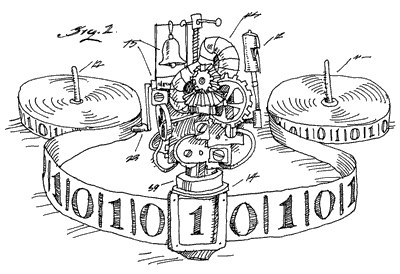
\includegraphics[width=0.2\textwidth]{turing-machine}\;\;}\end{minipage}}
\begin{frame}{Exploring the realizability model}
  \jnote{5}{
    The statement that every function~$\NN \to \NN$ is computable by a Turing
    machine (or equivalently, by a lambda term) is known as the \emph{formal
    Church--Turing thesis}. It is an example of a statement which is realizable
    but not provable in~HA\textsuperscript{$\omega$}.

    Many of the curious properties of the realizability model follow from the
    formal Church--Turing thesis. In fact, a slight generalization called the
    \emph{extended Church thesis} suffices to completely characterize the
    (provably) realizable statements:
    \[ \text{HA+ECT} \vdash \varphi \quad\text{iff}\quad
      \text{HA} \vdash (\realizes \varphi). \]

    In the realizability model built using lambda terms instead of Turing
    machines, the formal Church--Turing thesis fails. This is because of
    changed calling conventions: In the model built using lambda terms, a
    realizer for a statement of the form~``$\forall f\?N^N\_ \varphi(f)$'' is a
    lambda term~$e$ such that for every lambda term~$r$ computing a
    function~$f : \NN \to \NN$, the term $er$ is a realizer for~$\varphi(f)$.
    However, the term~$e$ cannot inspect the form (``source code'') of its
    argument.
  }

  \jnote{6}{
    Statement~5 is not a statement in the language of~HA or
    of~HA\textsuperscript{$\omega$}, but in an extension in which we can also
    support quotients (to make sense of the construction of the reals using
    equivalence classes of Cauchy sequences) or powersets (to support the
    construction using Dedekind cuts). A proper interpretation is possible in
    the category of assemblies or in the ef{}fective topos.

    An exposition of this continuity phenomenon is provided in
    \fixedhref{https://arxiv.org/pdf/2204.00948.pdf}{this survey paper}
    (Example~6 there).
  }

  \jnote{7}{
    By \emph{Markov's principle}, we mean the statement
    \[ \forall f\?N^N\_ (\neg\neg(\exists n\?N\_ f(n) = 0)) \Rightarrow
    (\exists n\?N\_ f(n) = 0). \]
    By the clauses for implication and negation, a number~$e$ is a realizer for
    a negated statement~$\neg\psi$ iff there is no realizer for~$\psi$:
    \begin{align*}
      e \realizes \neg\psi &\quad\text{iff}\quad
      \text{for every~$r \in \NN$ such that~$r \realizes \psi$, $e \cdot r
      \downarrow$ and~$e \cdot r \realizes \bot$} \\
      &\quad\text{iff}\quad \text{for every~$r \in \NN$ such that~$r \realizes \psi$, falsum holds} \\
      &\quad\text{iff}\quad \text{there is no number~$r \in \NN$ such that~$r \realizes \psi$} \\
      &\quad\text{iff}\quad \text{$\psi$ is not realized}
    \end{align*}
    In particular, if there exists a realizer for a negated statement at all,
    every number whatsoever is a realizer. As a consequence, \emph{realizers for
    negated statements are never informative;} and a number~$e$ is a realizer
    for~$\neg\neg\varphi$ iff~$\varphi$ is \emph{not~not} realizable. Hence a
    realizer for~$\neg\neg\varphi$ encodes the mere promise that somewhere,
    there is a realizer for~$\varphi$, without giving any indication how to
    find it.
  }

  \jnote{8}{
    By \emph{countable choice}, we mean the statement
    \[ (\forall x\?N\_ \exists y\?A\_ \varphi(x,y)) \Longrightarrow
      (\exists f\?A^N\_ \forall x\?N\_ \varphi(x,f(x))). \]
    Up to some repackaging, this statement is realized by the identity machine
    which simply outputs its input unchanged.

    Choice for higher type fails in the realizability model. For instance, the
    statement
    \[ (\forall f\?N^N\_ \exists y\?A\_ \varphi(f,y)) \Longrightarrow
      (\exists \theta\?A^{N^N}\_ \forall f\?N^N\_ \varphi(f,\theta(f))) \]
    is not realized. A realizer for the antecedent would be a machine which,
    given an index for a Turing machine computing a total function~$f : \NN \to
    \NN$, produces a code for a suitable element~$y$. However, this element~$y$
    might not only depend on the extensional input/output behavior of~$f$, but
    also on the specific index (source code), hence wouldn't describe an actual
    function on the set of computable functions~$\NN \to \NN$.

    This issue does not arise with countable choice, as natural numbers have
    unique codes.
  }

  \jnote{9}{
    Similar to Statement~5, Statement~8 can only be formulated in an extension
    of the formal language used here.

    It expresses that, up to unique isomorphism, there is just one model of
    Heyting arithmetic, namely the standard model. This is in stark contrast
    with the situation in classical mathematics, where Gödel's completeness
    theorem/Henkin term models can be used to concoct a host of nonstandard
    models.

    As a consequence, Peano arithmetic is ``quasi-inconsistent'' from the point
    of view of the realizability model, as it is consistent (being
    equiconsistent with HA) but does not admit a model (every model of PA is
    also a model of HA, but HA only has one model, and this does not validate
    the PA-theorem ``every Turing machine terminates or does not terminate'').

    Pointers to relevant literature are in
    \fixedhref{https://arxiv.org/pdf/2204.00948.pdf}{this survey paper}
    (Example~8 there). Also see
    \fixedhref{https://www.ps.uni-saarland.de/Publications/documents/HermesKirst_2022_An-Analysis.pdf}{the
    2022 paper by Marc Hermes and Dominik Kirst}, particularly also the final
    paragraph of their Section~8.1 which alludes to a result in a different
    direction.
  }

  \jnote{10}{
    As the examples illustrate, realizability and truth do not at all coincide:
    There are many statements which are realizable but not true from the point of
    view of classical mathematics (such as the formal Church--Turing thesis)
    and vice versa (such as the statement that every function~$\NN \to \NN$ has
    a zero or not).

    Within the realizability model, the situation is radically different.
    For every statement~$\varphi$, the statement~``$\varphi \Leftrightarrow
    (\realizes \varphi)$'' is realizable.

    The multiverse of models of constructive mathematics can be explored from
    the point of view of any base model, and from the point of view of the
    realizability model it looks quite different than from the point of view of
    classical mathematics.
  }

  \medskip
  \medskip
  \begin{tabular}{@{\!\!\!\!\!\!}l@{\,}llp{1.8cm}}
    \toprule
    & statement & classical? & realizable? \\
    \midrule
    \normalnumber{1} & Every number is prime or not prime. & \ccmark{}
    (trivially) & \ccmark \\
    \normalnumber{2} & After every number there is a prime. & \ccmark & \ccmark \\
    \normalnumber{3} & Every map $\NN \to \NN$ has a zero or not. & \ccmark{} (trivially) & \cxmark \\
    \normalnumber{4} & Every map $\NN \to \NN$ is computable. & \cxmark &
    \qswitch{4}{5}{\ccmark}\only<1-4>{\,} \visible<5->{(trivially)} \\
    \normalnumber{5} & Every map $\RR \to \RR$ is continuous. & \cxmark &
    \qswitch{5}{6}{\ccmark{} (if MP)} \\
    \normalnumber{6} & Markov's principle holds. & \ccmark{} (trivially) &
    \qswitch{6}{7}{\ccmark{} (if MP)} \\
    \normalnumber{7} & Countable choice holds. & \ccmark &
    \qswitch{7}{8}{\ccmark{} (always!)} \\
    \normalnumber{8} & Heyting arithmetic is categorical. & \cxmark &
    \qswitch{8}{9}{\ccmark{} (if MP)} \\
    \normalnumber{9} & A statement holds iff it is realized. & \cxmark &
    \qswitch{9}{10}{\ccmark} \\
    \bottomrule
  \end{tabular}
  \medskip

  \only<1>{\color{white}There is a machine which determines of any given
  number whether it is prime or not. \\\ \\\ }
  \only<2>{\expl{1}{There is a machine which determines of any given
  number whether it is prime or not. \\\ \\\ }}
  \only<3>{\expl{2}{There is a machine which, given a number~$n$, computes a
  prime larger than~$n$. \\\ \\\ }}
  \only<4>{\expl{3}{There is a machine which, given a machine
  computing a map~$f : \NN \to \NN$, determines whether~$f$ has a
  zero or not. \\\ \\\ }}
  \only<5>{\expl{4}{There is a machine which, given a machine
  computing a map~$f : \NN \to \NN$, outputs a machine
  computing~$f$. \\\ \\\ }}
  \only<6>{\ \\\ \\\ \\\ }
  \only<7>{\expl{6}{There is a machine which, given a machine
  computing a map~$f : \NN \to \NN$ and given the promise that it is \notnot
  the case that~$f$ has a zero, determines a zero of~$f$.}}
  \only<8>{\expl{7}{\justifying There is a machine which, given a machine
  computing for every~$x \in \NN$ some~$y \in A$ together with a realizer
  of~$\varphi(x,y)$, outputs a machine computing a suitable choice
  function~$\NN \to A$.}}
  \only<9>{\ \\\ \\\ \\\ }
\end{frame}}

\begin{frame}{Metatheory of Heyting arithmetic}
  \jnote{1}{
    Variants of the realizability model can be used to establish several
    metatheoretic properties of Heyting arithmetic. For the second and third
    properties, the keyword is ``realizability with proof''; for the fourth,
    using the variant of realizability built using System~T terms instead of
    Turing machines.
  }

  \begin{enumerate}
    \item \hil{Unprovability results:}
    \medskip

    There are instances of~\badbox{\textsc{lem}} which HA does not prove,
    such as ``every Turing machine terminates or does not terminate''.
    \bigskip

    \item \hil{Disjunction property:}
    \medskip

    If HA proves~$\varphi \vee \psi$, then HA
    proves~$\varphi$ or HA proves~$\psi$.
    \bigskip

    \item \hil{Existence property:}
    \medskip

    If HA proves~$\exists n\?N\_ \varphi(n)$, then there is a number~$n_0 \in
    \NN$ such that HA proves~$\varphi(\underline{n_0})$.
    \bigskip

    \item \hil{Growth rate:}
    \medskip\justifying

    If HA proves~$\forall x\?N\_ \exists y\?N\_ \varphi(x,y)$,
    then there exists a \hil{higher primitive recursive} function $f_0 : \NN
    \to \NN$ such that for all~$x_0 \in \NN$, HA proves
    $\varphi(\underline{x_0}, \underline{f_0(x_0)})$.
  \end{enumerate}
\end{frame}

\begin{frame}{Range of machine models}
  \jnote{1-}{
    Infinite time Turing machines were introduced
    \fixedhref{https://arxiv.org/abs/math/9808093}{by Joel David Hamkins and
    Andy Lewis}. Unlike ordinary Turing machines, they can carry out ``more
    than infinitely many computational steps''. Where an ordinary Turing
    machine fails to terminate, an infinite time Turing machine is put on
    day~$\omega$ into a special limit state and can then meaningfully continue.

    All functions in Gödel's System~T are unconditionally total. Hence
    unbounded search cannot be implemented in System~T.

    The idea to apply realizability to machines in the real world is
    \fixedhref{http://math.andrej.com/2014/03/04/intuitionistic-mathematics-and-realizability-in-the-physical-world/}{due to Andrej Bauer}.
  }

  \begin{enumerate}
    \item \hil{Turing machines}

    \visible<2->{``Every map $\NN \to \NN$ is computable'' is realized by
    \textsf{cat}.}
    \medskip

    \item \hil{Untyped lambda calculus}

    \visible<3->{``Every map $\NN \to \NN$ is computable'' is \emph{not}
    realized.}
    \medskip

    \item \hil{Infinite-time Turing machines}

    \visible<4->{\mbox{``Every map $\NN \to \NN$ has a zero or not'' is realized by
    infinite search.}\\[0em]}
    \medskip

    \item \hil{Gödel's System T}

    \visible<5->{Markov's principle is not realized.}
    \medskip

    \item \hil{Machines in the real world} -- \emph{philosophical}

    \justifying
    \visible<6->{``Every map $\RR \to \RR$ is continuous'' is realized if,
    in the physical world, only finitely many computational
    steps can be carried out in finite time and if it is possible to form
    tamper-free private communication channels.}
  \end{enumerate}
\end{frame}


\section{Proof transformations}

\addtocounter{framenumber}{-1}
\begin{frame}[plain]\frametitle{A classical logic fairy tale}
  \vspace*{-0.5em}
  \begin{changemargin}{-1em}{-1em}
    \setlength{\columnsep}{15pt}
    \begin{multicols}{2}
      \justifying
      \scriptsize

      \textbf{Narrator.} Once upon a time, in a kingdom far, far away, the
      queen of the land and of all Möbius strips called for her royal
      philosopher.

      \textbf{Queen.} Philosopher! I ask you to carry out the following order.
      Get me the Philosopher's Stone, or alternatively find out how one could
      produce arbitrary amounts of gold with it!

      \textbf{Philosopher.} But my queen! I haven't studied anything useful!
      How could I fulfill this order?

      \textbf{Queen.} That is not my concern. I'll see you again tomorrow.
      Should you not accomplish the task, I will take your head off.

      \textbf{Narrator.} After a long and wakeful night the philosopher was
      called to the queen again.

      \textbf{Queen.} Tell me! What do you have to report?

      \textbf{Philosopher.} It was not easy and I needed to follow lots of
      obscure references, but finally I actually found out how to use the
      Philosopher's Stone to produce arbitrary amounts of gold. But only I can
      conduct this procedure, your royal highness.

      \textbf{Queen.}
      Alright. So be it.

      \textbf{Narrator.} And so years passed by, during which the philosopher
      imagined herself to be safe. The queen searched for the stone on her own,
      but as long as she hadn't found it, the philosopher didn't need to worry.
      Yet one day the impossible happened: The queen has found the stone! And
      promptly called for her philosopher.

      \textbf{Queen.} Philosopher, look! I have found the Philosopher's Stone!
      Now live up to your promise! \emph{[She hands over the stone.]}

      \textbf{Philosopher.} Thank you. \emph{[She inspects the stone.]} This is
      indeed the Philosopher's Stone. Many years ago you asked me to either
      acquire the Philosopher's Stone or find out how to produce arbitrary
      amounts of gold using it. Now it's my pleasure to present to you the
      Philosopher's Stone. \emph{[She returns the stone.]}
    \end{multicols}
  \end{changemargin}

  \jnote{1}{
    Adapted from
    \fixedhref{http://blog.ezyang.com/2013/04/a-classical-logic-fairy-tale/}{Edward
    Yang's blog}.
  }
\end{frame}

\begin{frame}
  \centering\bigskip
  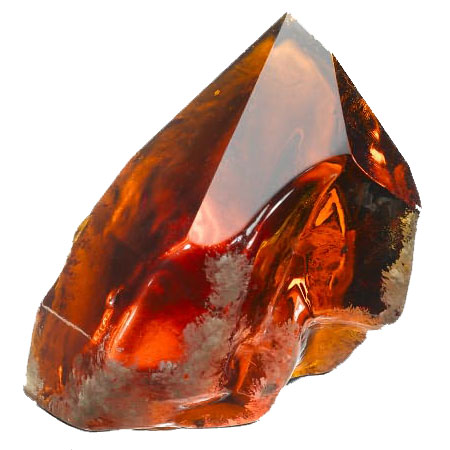
\includegraphics[height=9.5em]{philosophers-stone}
  \medskip

  \large Lecture II: \\
  \hil{Proof transformations}

  \normalsize

  \emph{for extracting constructive proofs from classical proofs}
\end{frame}

\begin{frame}{A case study in double negation}
  \jnote{2-4}{
    The two displayed proofs seem to be devoid of computational content:
    Computationally, it is neither possible to determine the minimal element of
    an infinite sequence nor to determine whether a binary sequence contains
    infinitely many zeros or infinitely many ones. These claims have no
    realizer.

    However, contrary to expectations, the two proofs do contain an obscured
    constructive core, and this core can be uncovered by the two logical
    metatheorems presented in this lecture, the double-negation embedding and
    \emph{Friedman's trick}. Details are in Thierry Coquand's
    \fixedhref{https://www.lama.univ-savoie.fr/pagesmembres/ruyer/divers/lecturearticles/coquand/cor3.ps}{Computational
    Content of Classical Logic}.
  }

  \jnote{3-4}{
    To set the stage, we analyze the lemma used in the first proof. The
    statement ``every inhabited set of natural numbers contains a minimal
    element'' is not realizable and hence does not directly have
    computational content. In fact, this statement is equivalent to the law of
    excluded middle. Correspondingly, it seems that proofs using it cannot ever
    be constructivized. However, as we will see, much more important for
    extraction of constructive content is the form of the asserted end results than
    the form of auxiliary lemmas used in a proof.
  }

  \jnote{5-}{
    A set~$X$ of natural numbers is \emph{detachable} if and only if for every
    number~$n \in \NN$, either~$n \in X$ or~$n \not\in X$. In classical
    mathematics, every set of natural numbers is detachable. Constructively,
    detachability is a nontrivial and computationally meaningful condition. A
    realizer for detachability of a set~$X$ is a machine which reads a
    number~$n$ as input and determines whether~$n$ belongs to~$X$ or not
    (outputting also corresponding realizers).
  }

  \jnote{7-}{
    Instead of strengthening the assumption, we can also weaken the conclusion.
    Statement~3 merely asserts that it is impossible that no minimum exists.
    The \emph{double-negation embedding} reviewed on the next slide explains
    why it can be expected a priori that this weakening allows us to give a
    constructive proof.
  }

  \vspace*{-0.8em}
  \mbox{How to extract \good{constructive proofs} from
  \bad{classical proofs} as the following?}

  \begin{enumerate}
    \item \textbf{Thm.} Every infinite sequence~$\alpha : \NN \to \NN$ is \emph{good}
    in that there are numbers~$i < j$ such that~$\alpha(i) \leq \alpha(j)$.
    \medskip

    {\emph{Proof.} By~\badbox{\textsc{lem}}, there is a minimal value~$\alpha(i)$.
    Set~$j \defeq i + 1$.\par}
    \medskip
    \pause

    \item \textbf{Thm.} Every infinite binary sequence contains repeated terms.
    \medskip

    {\emph{Proof.} By the \bad{infinite box principle},
    infinitely many terms are zeros or are ones. In either case the claim
    follows.\par}
    \pause
  \end{enumerate}
  \vspace*{-0.7em}

  \grayline

  \textbf{Lemma.} Let~$X$ be an inhabited set of natural numbers.
  \begin{enumerate}
    \item Assuming~\badbox{\textsc{lem}}, the set~$X$ contains a minimal element.
    \item<5-> If~$X$ is \hil{detachable}, then~$X$ contains a minimal element.
    \item<7-> It is \hil{not~not} the case that~$X$ contains a minimal element.
  \end{enumerate}

  \justifying
  \only<1-3>{\ \\\ \\\ \\\ }
  \only<4-5>{\emph{Proof of~\normalnumber{1}.} There is some~$n \in X$.
  By~\badbox{\textsc{lem}}, either~$\exists k \in X\_ k < n$ \\ or not. In the
  first case, we continue by induction. Else~$n$ is minimal.\\\ \par}
  \only<6-7>{\mbox{\emph{Proof of~\normalnumber{2}.} There is some~$n \in X$.
  By~\good{assumption}, either~$\exists k \in X\_ k < n$} or not. In the
  first case, we continue by induction. Else~$n$ is minimal.\\\ \par}
  \only<8>{\emph{Proof of~\normalnumber{3}.} There is some~$n \in X$. Assume that~$X$ does not
  contain a minimum. Then it is not the case that~$\exists k \in X\_ k <
  n$, as else~$\bot$ by induction. Hence~$n$ is minimal. This is a
  contradiction.\par}
\end{frame}

\newcommand{\hnegneg}{\hil{$\neg\neg$}}
\newcommand{\negg}{{\neg}\!\!\!{\neg}}
\newcommand{\neggv}{{\neg}\!\!\!\phantom{{\neg}}}
\newcommand{\bott}{\bot\!\!\!\!\bot}
\newcommand{\bottv}{\bot\!\!\!\!\phantom{\bot}}

\begin{frame}{The double-negation embedding}
  \jnote{1-3}{
    Minimal logic is intuitionistic logic minus \emph{ex falsum quodlibet}
    ($\bot \seq{\vec x} \varphi$).

    The double-negation embedding builds on a fundamental
    observation: While the law
    of excluded middle is not available in minimal or intuitionistic logic, the double
    negation of every instance is---for every formula~$\varphi$, the formula
    $\neg\neg(\varphi \vee \neg\varphi)$
    is an intuitionistic tautology:

    \begin{quote}
      In order to show~$\neg\neg(\varphi \vee \neg\varphi)$,
      assume~$\neg(\varphi \vee \neg\varphi)$ and deduce~$\bot$.

      As a preparatory step, we verify~$\neg\varphi$: If~$\varphi$, then in
      particular~$\varphi \vee \neg\varphi$, hence~$\bot$ by assumption.

      Having established~$\neg\varphi$, we notice that also~$\varphi \vee
      \neg\varphi$, hence~$\bot$ by assumption.
    \end{quote}

    \vspace*{-0.6em}
    Also, a doubly negated statement is not a dead end. Instead, we can
    continue reasoning, by the following tautology (``Kleisli extension'',
    ``monadic bind'', ``nucleus axiom''):

    \vspace*{-1.6em}
    \[ (\neg\neg\varphi \wedge (\varphi \Rightarrow \neg\neg\psi))
    \Longrightarrow \neg\neg\psi \]
  }

  \jnote{3}{
    \vspace*{-0.8em}
    The three parts of the theorem are each proven by induction, on the
    structure of~$\varphi$ for the first two parts and on the structure of
    derivations for the third part. Carrying this out is an instructive
    exercise!
  }

  \jnote{4}{
    The corollary follows from the theorem because HA proves the
    double-negation translation of every axiom of PA. For instance, the
    translation of the axiom
    \[ \forall x\?N\_ x + 0 = x \]
    is
    \[ \forall x\?N\_ \neg\neg(x + 0 = x), \]
    and this weaker statement is provable thanks to the intuitionistic (even
    minimal) tautology~$\varphi \Rightarrow \neg\neg\varphi$.

    Similarly, the translation of an instance of the induction scheme
    \[
      \varphi(0) \wedge \bigl(\forall x\?N\_ \varphi(x) \Rightarrow
      \varphi(S(x))\bigr) \quad\Longrightarrow\quad \forall x\?N\_ \varphi(x)
    \]
    is again an instance of the induction scheme:
    \[
      \varphi(0)^{\neg\neg} \wedge \bigl(\forall x\?N\_ \varphi(x)^{\neg\neg} \Rightarrow
      \varphi(S(x))^{\neg\neg}\bigr) \quad\Longrightarrow\quad \forall x\?N\_
      \varphi(x)^{\neg\neg}
    \]
  }

  \jnote{5}{
    Live demo with
    \fixedhref{https://agdapad.quasicoherent.io/~AgdaPadova/html/Dickson-pc2022.html}{Agda
    code for the theorem on all infinite sequences of natural numbers being
    good}:

    \begin{enumerate}
    \item\justifying The first proof there implements the classical proof,
    postulating the law of excluded middle as an unprovable axiom. Thereby Agda
    can verify the classical proof to be correct, however trying to run the
    proof will get stuck on the postulated \textsc{lem}-oracle.

    \item The second proof rewrites the statement of the theorem and its proof
    by the double-negation translation. The result is a constructive proof
    which doesn't rely on postulates; however there is still no direct
    computational content, as the asserted claim is a (doubly) negated
    statement.

    \item In a logical sleight of hand, the third proof imports the
    second proof but specializes~$\bot$, which was an arbitrary constant there,
    to the asserted claim. The tautology~$\negg\negg\bott \Rightarrow \bott$ of
    minimal logic is then used to escape the double-negation monad and obtain a
    constructive proof of the full result.
    \end{enumerate}
  }

  \justifying
  \vspace*{-1em}
  \small
  \textbf{Def.} For formulas over a fixed first-order signature, the
  \hil{$\neg\neg$-translation} $\varphi \mapsto \varphi^{\neg\neg}$ is defined
  by the following clauses.
  \begin{align*}
    (\varphi_\text{atomic})^{\neg\neg} &\defeqv \hnegneg \varphi_\text{atomic} &
    (\varphi \Rightarrow \psi)^{\neg\neg} &\defeqv (\varphi^{\neg\neg} \Rightarrow \psi^{\neg\neg}) \\
    \bot^{\neg\neg} &\defeqv \hnegneg\bot &
    \top^{\neg\neg} &\defeqv \top \\
    (\varphi \vee \psi)^{\neg\neg} &\defeqv \hnegneg(\varphi^{\neg\neg} \vee \psi^{\neg\neg}) &
    (\varphi \wedge \psi)^{\neg\neg} &\defeqv (\varphi^{\neg\neg} \wedge \psi^{\neg\neg}) \\
    (\exists x\?X\_ \varphi)^{\neg\neg} &\defeqv \hnegneg{(\exists x\?X\_ \varphi^{\neg\neg})} &
    (\forall x\?X\_ \varphi)^{\neg\neg} &\defeqv (\forall x\?X\_ \varphi^{\neg\neg}) \\
  \end{align*}
  \vspace*{-3em}

  \mbox{\textbf{Ex.} $(\forall a{:}X\_\! \exists b{:}X\_\! a = b \vee \ldots)^{\neg\neg}
  \equiv (\forall a{:}X\_\! \hnegneg\exists b{:}X\_\! \hnegneg(\hnegneg(a=b) \vee
  (\ldots)^{\neg\neg})).$}
  \pause

  \textbf{Prop.} Classically, $\varphi \Leftrightarrow \varphi^{\neg\neg}$.
  \pause
  \vspace*{-0.5em}

  \grayline

  \textbf{Thm.} For every formula~$\varphi$ and set of formulas~$\Gamma$:
  \vspace*{-0.6em}
  \begin{enumerate}
    \item Minimally, $\neg\neg(\varphi^{\neg\neg}) \Rightarrow
    \varphi^{\neg\neg}$.
    \item Minimally, $\varphi^{\neg\neg} \Leftrightarrow \neg\neg\varphi$ in
    case that~$\varphi$ is geometric
    ($R{\top}{\bot}{\wedge}{\vee}{\exists}{\bigvee}$).
    \item If~$\Gamma$ entails~$\varphi$ classically,
    then~$\Gamma^{\neg\neg}$ entails~$\varphi^{\neg\neg}$ minimally.
  \end{enumerate}
  \pause
  \vspace*{-0.3em}

  \textbf{Cor.} If PA proves~$\varphi$, then~HA proves~$\varphi^{\neg\neg}$.
  \pause

  \textbf{Rem.} Theorem and corollary hold for every \hil{local
  operator}~$\nabla$ in place of~$\neg\neg$, in particular for~$\negg\negg\varphi \defeq
  ((\varphi \Rightarrow \bott) \Rightarrow \bott)$ for some arbitrary
  formula~$\bott$.
\end{frame}

\newcommand{\negx}{\hil{${\only<1>{\neggv}\only<2->{\negg}}$}}
\newcommand{\botx}{\hil{${\only<1>{\bottv}\only<2>{\bott}\only<3->{\beta}}$}}

\begin{frame}{Barr's theorem / Friedman's trick / A-translation}
  \jnote{4}{
    The proof transformation for~``$3 \Rightarrow 2$'' is explicit in
    nature, feasible in practice and increases the proof length only
    polynomially. There is also an
    \fixedhref{https://drops.dagstuhl.de/opus/volltexte/2022/16776/pdf/LIPIcs-TYPES-2021-7.pdf}{intriguing
    alternative approach by Giulio Fellin, Sara Negri and Eugenio Orlandelli}
    employing cut elimination (thereby increasing the proof length
    substantially, but conceptually beneficial in other aspects). Furthermore,
    this metatheorem can also be cast in semantic terms:

    Every Grothendieck topos admits a cover (a surjective geometric morphism from
    another Grothendieck topos) by a Grothendieck topos which is boolean. This
    can be obtained by first adjoining a \emph{generic proposition}~$\chi$ and then
    taking sheaves with respect to the modality~$(({\cdot} \Rightarrow \chi)
    \Rightarrow \chi)$.

    Applied to the classifying topos of~$\Gamma$, this insight yields a proof
    of~``$3 \Rightarrow 0$'', since pullback along surjective geometric
    morphisms reflects validity of geometric sequents.

    Furthermore, every Grothendieck topos admits a cover by a Grothendieck
    topos over a complete Boolean algebra. Assuming Zorn's lemma in the
    metatheory, this topos validates~\textsc{lem} and~\textsc{zorn},
    hence~\textsc{ac}. This shows~``$4 \Rightarrow 0$''.

    An introduction to topos-theoretic generic models with a view towards
    applications in constructive commutative algebra is contained in
    \fixedhref{https://arxiv.org/abs/2012.13850}{this survey}.
    \vspace*{2em}
  }

  \textbf{Thm.} Let~$\Gamma$ be a set of geometric sequents over a fixed
  signature. Let~$\sigma$ be a geometric sequent. Then the following are
  equivalent:
  \begin{enumerate}
    \addtocounter{enumi}{-1}
    \item $\sigma$ holds for the \good{generic model} of~$\Gamma$ (in its
    classifying topos).
    \item $\sigma$ is provable from~$\Gamma$ in \good{geometric logic}.
    \item $\sigma$ is provable from~$\Gamma$ in \good{intuitionistic logic}.
    \item $\sigma$ is provable from~$\Gamma$ in \bad{classical logic}.
    \item (Assuming \badbox{\textsc{zorn}}) $\sigma$ is provable from~$\Gamma$ in
    \bad{classical logic with~\textsc{ac}}.
  \end{enumerate}

  \emph{Proof of~``\,\,$\normalnumber{3} \Rightarrow \normalnumber{2}$''.}
  Write~$\sigma \equiv (\alpha \seq{\vec x} \beta)$. Then intuitionistically,
  \[ \alpha \Longrightarrow
    \negx\negx\alpha \Longleftrightarrow
    \alpha^{\negx\negx} \Longrightarrow
    \beta^{\negx\negx} \Longleftrightarrow
    \negx\negx\beta \equiv
    ((\beta{\Longrightarrow}\botx){\Rightarrow}\botx)
    \visible<4->{\Longrightarrow \beta.}
  \]
\end{frame}


\section{Constructive proofs from invalid proofs}

\begin{frame}
  \jnote{3}{
    \textbf{Thm. 1.} From every proof~$p$ of a statement~$\varphi$ such that
    \vspace*{-0.5em}
    \begin{enumerate}
      \item the assertion~$\varphi$ is a first-order statement,
      \item the proof~$p$ is constructive,
      \item the proof~$p$ is formulated in a certain higher-order system (in
      particular, the proof may, unlike its end result, freely employ
      higher-order notions) and
      \item for a certain set~$X$ appearing in~$p$, the proof assumes that~$X$
      is countable,
    \end{enumerate}
    \vspace*{-0.5em}
    a constructive proof of the same statement~$\varphi$, set in the same
    system, but \emph{without requiring the countability assumption} can be
    extracted.
  }

  \jnote{4}{
    \textbf{Thm. 2.} From every proof~$p$ of a statement~$\varphi$ such that
    \vspace*{-0.5em}
    \begin{enumerate}
      \item the assertion~$\varphi$ is a geometric implication,
      \item the proof~$p$ is classical (constructive + \textsc{lem}, but still no
      \textsc{zorn}),
      \item the proof~$p$ is formulated in a certain higher-order system (in
      particular, the proof may, unlike its end result, freely employ
      higher-order notions) and
      \item for a certain set~$X$ appearing in~$p$, the proof assumes that~$X$
      is countable,
    \end{enumerate}
    \vspace*{-0.5em}
    a classical proof of the same statement~$\varphi$, set in the same
    system, but \emph{without requiring the countability assumption} can be
    extracted.
  }

  \centering\bigskip
  
\includegraphics[height=9.5em]{phantoms}
  \medskip

  \large Lecture III: \\
  \hil{Extracting constructive proofs from invalid* proofs}

  \normalsize

  \visible<3->{\emph{* higher-order proofs of first-order statements using the assumption \\
  that a given (perhaps uncountable) set is countable}}

  \pause
  \vspace*{1em}
  \mbox{\begin{minipage}{0.15\textwidth}
    \centering\small
    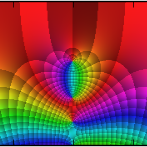
\includegraphics[height=5em]{zeta-function} \\
    $\mathbb{C}$
  \end{minipage}\quad
  \begin{minipage}{0.20\textwidth}
    \centering\small
    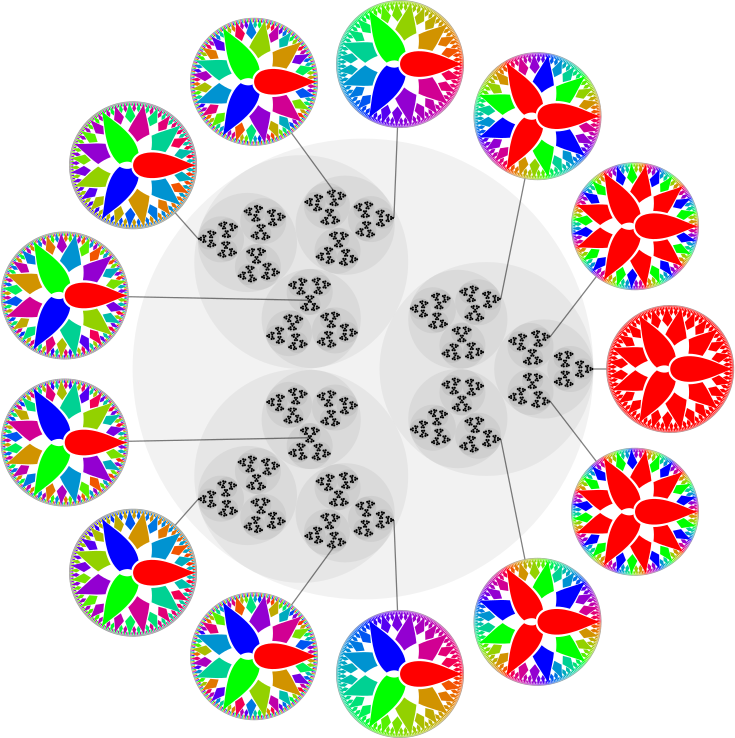
\includegraphics[height=5em]{3-adic-numbers} \\
    $\mathbb{Q}_p$
  \end{minipage}\quad
  \begin{minipage}{0.20\textwidth}
    \centering\small
    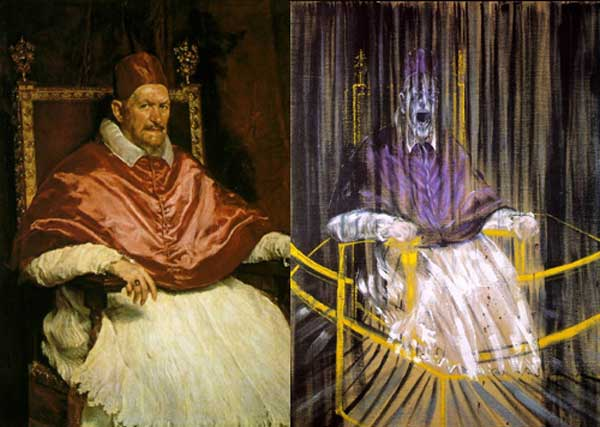
\includegraphics[height=5em]{bruyn-pope} \\
    $\mathbb{F}_1$
  \end{minipage}\quad
  \begin{minipage}{0.42\textwidth}
    \centering\small
    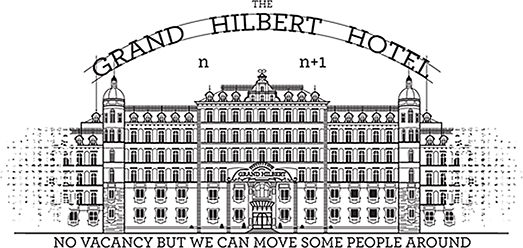
\includegraphics[height=5em]{hilbert-hotel} \\
    $\infty$
  \end{minipage}}
\end{frame}

\begin{frame}{A quantifier for finite approximations}
  Let~$X$ be a (perhaps uncountable) set. By a \hil{finite approximation} to a
  surjection~$\NN \twoheadrightarrow X$, we mean a \hil{finite list} of
  elements of~$X$. Notation:

  \begin{itemize}
    \item empty list: $[]$
    \item extension: $[x_1,\ldots,x_n] ::^r x_{n+1} = [x_1,\ldots,x_n,x_{n+1}]$
    \item refinement relation: $[x_1,\ldots,x_n,x_{n+1},\ldots,x_{n+m}] \preceq [x_1,\ldots,x_n]$
    \item element access: $\sigma[i] = \text{element at position~$i$
    in~$\sigma$}$
  \end{itemize}
  \justifying
  \pause

  For monotone predicates~$P$ of finite lists, we introduce
  a \hil{quantifier}~$\nabla$ such that~``$\nabla^{\tau \preceq \sigma}\_
  P(\tau)$'' expresses that \hil{no matter how~$\sigma$ evolves to a
  better approximation~$\tau$, eventually~$P(\tau)$ will hold}.
  \[
    \infer[{\text{\scriptsize$(\sigma \in X^*)$}}]{\nabla^{\tau \preceq \sigma}\_ P(\tau)}{P(\sigma)}
    \qquad
    \infer[{\text{\scriptsize$(\sigma \in X^*)$}}]{\nabla^{\tau \preceq
    \sigma}\_ P(\tau)}{\forall^{x \in X}\_\ \nabla^{\tau
    \preceq (\sigma ::^r x)}\_ P(\tau)}
  \]
  \[
    \infer[{\text{\scriptsize$(\sigma \in X^*, a \in X)$}}]{\nabla^{\tau
    \preceq \sigma}\_ P(\tau)}{\forall^{\tau \preceq \sigma}\_\
    a \in \tau \Rightarrow \nabla^{\upsilon \preceq \tau}\_ P(\upsilon)}
  \]
\end{frame}

\newcommand{\hnabla}{\hil{$\nabla$}}
\newcommand{\genalpha}{\mbox{$\hspace{0.12em}\shortmid\hspace{-0.62em}\alpha$}}

\begin{frame}{The generic surjection}
  \vspace*{-0.6em}
  \justifying
  \textbf{Def.} The \hil{$\nabla$-translation} $\varphi \mapsto
  \varphi^{\nabla}$ into formulas with a free variable $\sigma : X^*$ (denoting
  the \hil{current stage}) is defined by the following clauses.
  {\small
  \begin{align*}
    (\varphi_\text{atomic})^{\nabla} &\defeqv \hnabla^{\tau \preceq \sigma}\_
    \varphi_\text{atomic} \\
    \bot^{\nabla} &\defeqv \hnabla^{\tau\preceq\sigma}\_ \bot \\
    (\varphi \vee \psi)^{\nabla} &\defeqv \hnabla^{\tau\preceq\sigma}\_
      (\varphi^{\nabla}[\tau/\sigma] \vee \psi^{\nabla}[\tau/\sigma]) \\
    (\exists^{x\?X}\_ \varphi)^{\nabla} &\defeqv
    \hnabla^{\tau\preceq\sigma}\_(\exists^{x\?X}\_ \varphi^{\nabla}[\tau/\sigma]) \\
    (\varphi \Rightarrow \psi)^{\nabla} &\defeqv
      \forall^{\tau\preceq\sigma}\_ (\varphi^{\nabla}[\tau/\sigma] \Rightarrow
      \psi^{\nabla}[\tau/\sigma]) \\
    \top^{\nabla} &\defeqv \top \\
    (\varphi \wedge \psi)^{\nabla} &\defeqv (\varphi^{\nabla} \wedge \psi^{\nabla}) \\
    (\forall^{x\?X}\_ \varphi)^{\nabla} &\defeqv
      (\forall^{x\?X}\_
      \varphi^{\nabla}[\sigma/\tau]) \\
    (\genalpha(n){=}x)^\nabla &\defeqv
      (\hnabla^{\tau\preceq\sigma}\_ (\textsf{len}(\tau) > n \wedge \tau[n] = x))
  \end{align*}}

  \vspace*{-0.3em}
  \textbf{Ex.} $(\forall^{x\?X}\_ \exists^{n\?\NN}\_ \genalpha(n){=}x)^\nabla
  \equiv$ \\
  $\qquad\qquad
    (\forall^{x\?X}\_ \nabla^{\tau\preceq\sigma}\_
    \exists^{n\?\NN}\_
    \nabla^{\upsilon\preceq\tau}\_ (\textsf{len}(\upsilon) > n \wedge \upsilon[n] = x)).$

  \vspace*{-0.3em}
  \textbf{Thm.} [Joyal--Tierney 1984] For \hil{first-order} formulas~$\varphi$
  not referring to~$\genalpha$, $\varphi^\nabla \Rightarrow \varphi$
  intuitionistically.
\end{frame}

\end{document}

start:
- infinitude of primes
- Dickson's lemma
- "Every constructive theorem has a computable witness."
- induction = recursion, Markov = unbounded search, ...
- side effects
- applications:
  - integrated developments (for instance SAT checking)
  - metatheory of constructive systems
  - philosophy
  - exploring computability theory

definition:
- HA
- TM
- realizability (as formalization of BKH)
- proof

examples:
- as in filmat paper
  - also with lambda terms!

special kinds of statements:
- negated: uninformative
- double negation
- Π⁰₁

metatheory of HA:
- disjunction property
- existence property
- unprovability of (for instance) halting
- growth rate

variants:
- ITTM
- real world
- completion to Eff

----

- play
- double-negation embedding
- Friedman's trick
- perhaps in Agda

\begin{block}{}
  \justifying
  \textbf{Thm.}
  Every pair of infinite sequences~$\alpha,\beta : \NN \to \NN$ is \emph{good} in that
  there are~$i < j$ such that~$\alpha(i)
  \leq \alpha(j)$ and~$\beta(i) \leq \beta(j)$.
\end{block}
\vspace*{-0.6em}
{\small\emph{Proof.} By~\badbox{\textsc{lem}}+\badbox{\textsc{dc}}, there is a
monotonic subsequence
\[ \alpha(i_0) \leq \alpha(i_1) \leq \alpha(i_2) \leq \cdots \]
with~$i_0 < i_1 < \cdots$. By~\badbox{\textsc{lem}}, there is a minimal
value~$\beta(i_{k_0})$ among all values of~$(\beta(i_k))_k$. Then
$\alpha(i_{k_0}) \leq \alpha(i_{k_0+1})$ and
$\beta(i_{k_0}) \leq \beta(i_{k_0+1})$. \qed
\par}


Claim: (∃n ∈ X) ⇒ X has a minimum.

Classical proof:
By LEM, ∃(k ∈ X). k < n or not.
In the first case, we conclude by induction.
In the second case, we conclude that n is minimal:
  Given k ∈ X, we have k < n or n ≤ k.
  In the first case, ⊥ and hence conclusion.
  In the second case, good.

Translated proof:
Assume that X does not have a minimum, show ⊥.
May conclude that ¬(∃(k ∈ X). k < n). For else, X inhabited by <n, so ⊥ by induction.
Thus n is a minimum:
  Given k ∈ X, we have k < n or n ≤ k.
  In the first case, ⊥ and hence conclusion.
  In the second case, good.

\begin{tabular}{ll@{\qquad\qquad}ll}
  \toprule
  $\varphi$ & $\varphi^{\neg\neg}$ &
  $\varphi$ & $\varphi^{\neg\neg}$ \\\midrule
  $\alpha_\text{atomic}$ & $\hnegneg \alpha_\text{atomic}$ &
  $\alpha \Rightarrow \beta$ & $\alpha^{\nabla} \Rightarrow \beta^{\nabla}$ \\
  $\bot^{\neg\neg}$ & $\hnegneg\bot$ &
  $\top^{\neg\neg}$ & $\top$ \\
  $\alpha \vee \beta$ & $\hnegneg(\alpha^{\neg\neg} \vee \beta^{\neg\neg})$ &
  $\alpha \wedge \beta$ & $\alpha^{\neg\neg} \wedge \beta^{\neg\neg}$ \\
  \bottomrule
\end{tabular}
